\documentclass{beamer}
\usetheme{default}
\usepackage{chemformula}
\usepackage[super,sort&compress,comma]{natbib}

\title{February Update}
\author{Ben Goldmann}
\date{\today}

\usepackage{caption}
\captionsetup[figure]{labelformat=empty}
\captionsetup[table]{labelformat=empty}

\begin{document}

\begin{frame}
\titlepage
\end{frame}

\begin{frame}
\frametitle{Stability of Alkaline Earth Metal Ion Buckingham Potentials in \ch{Na3OCl}}

\begin{figure}
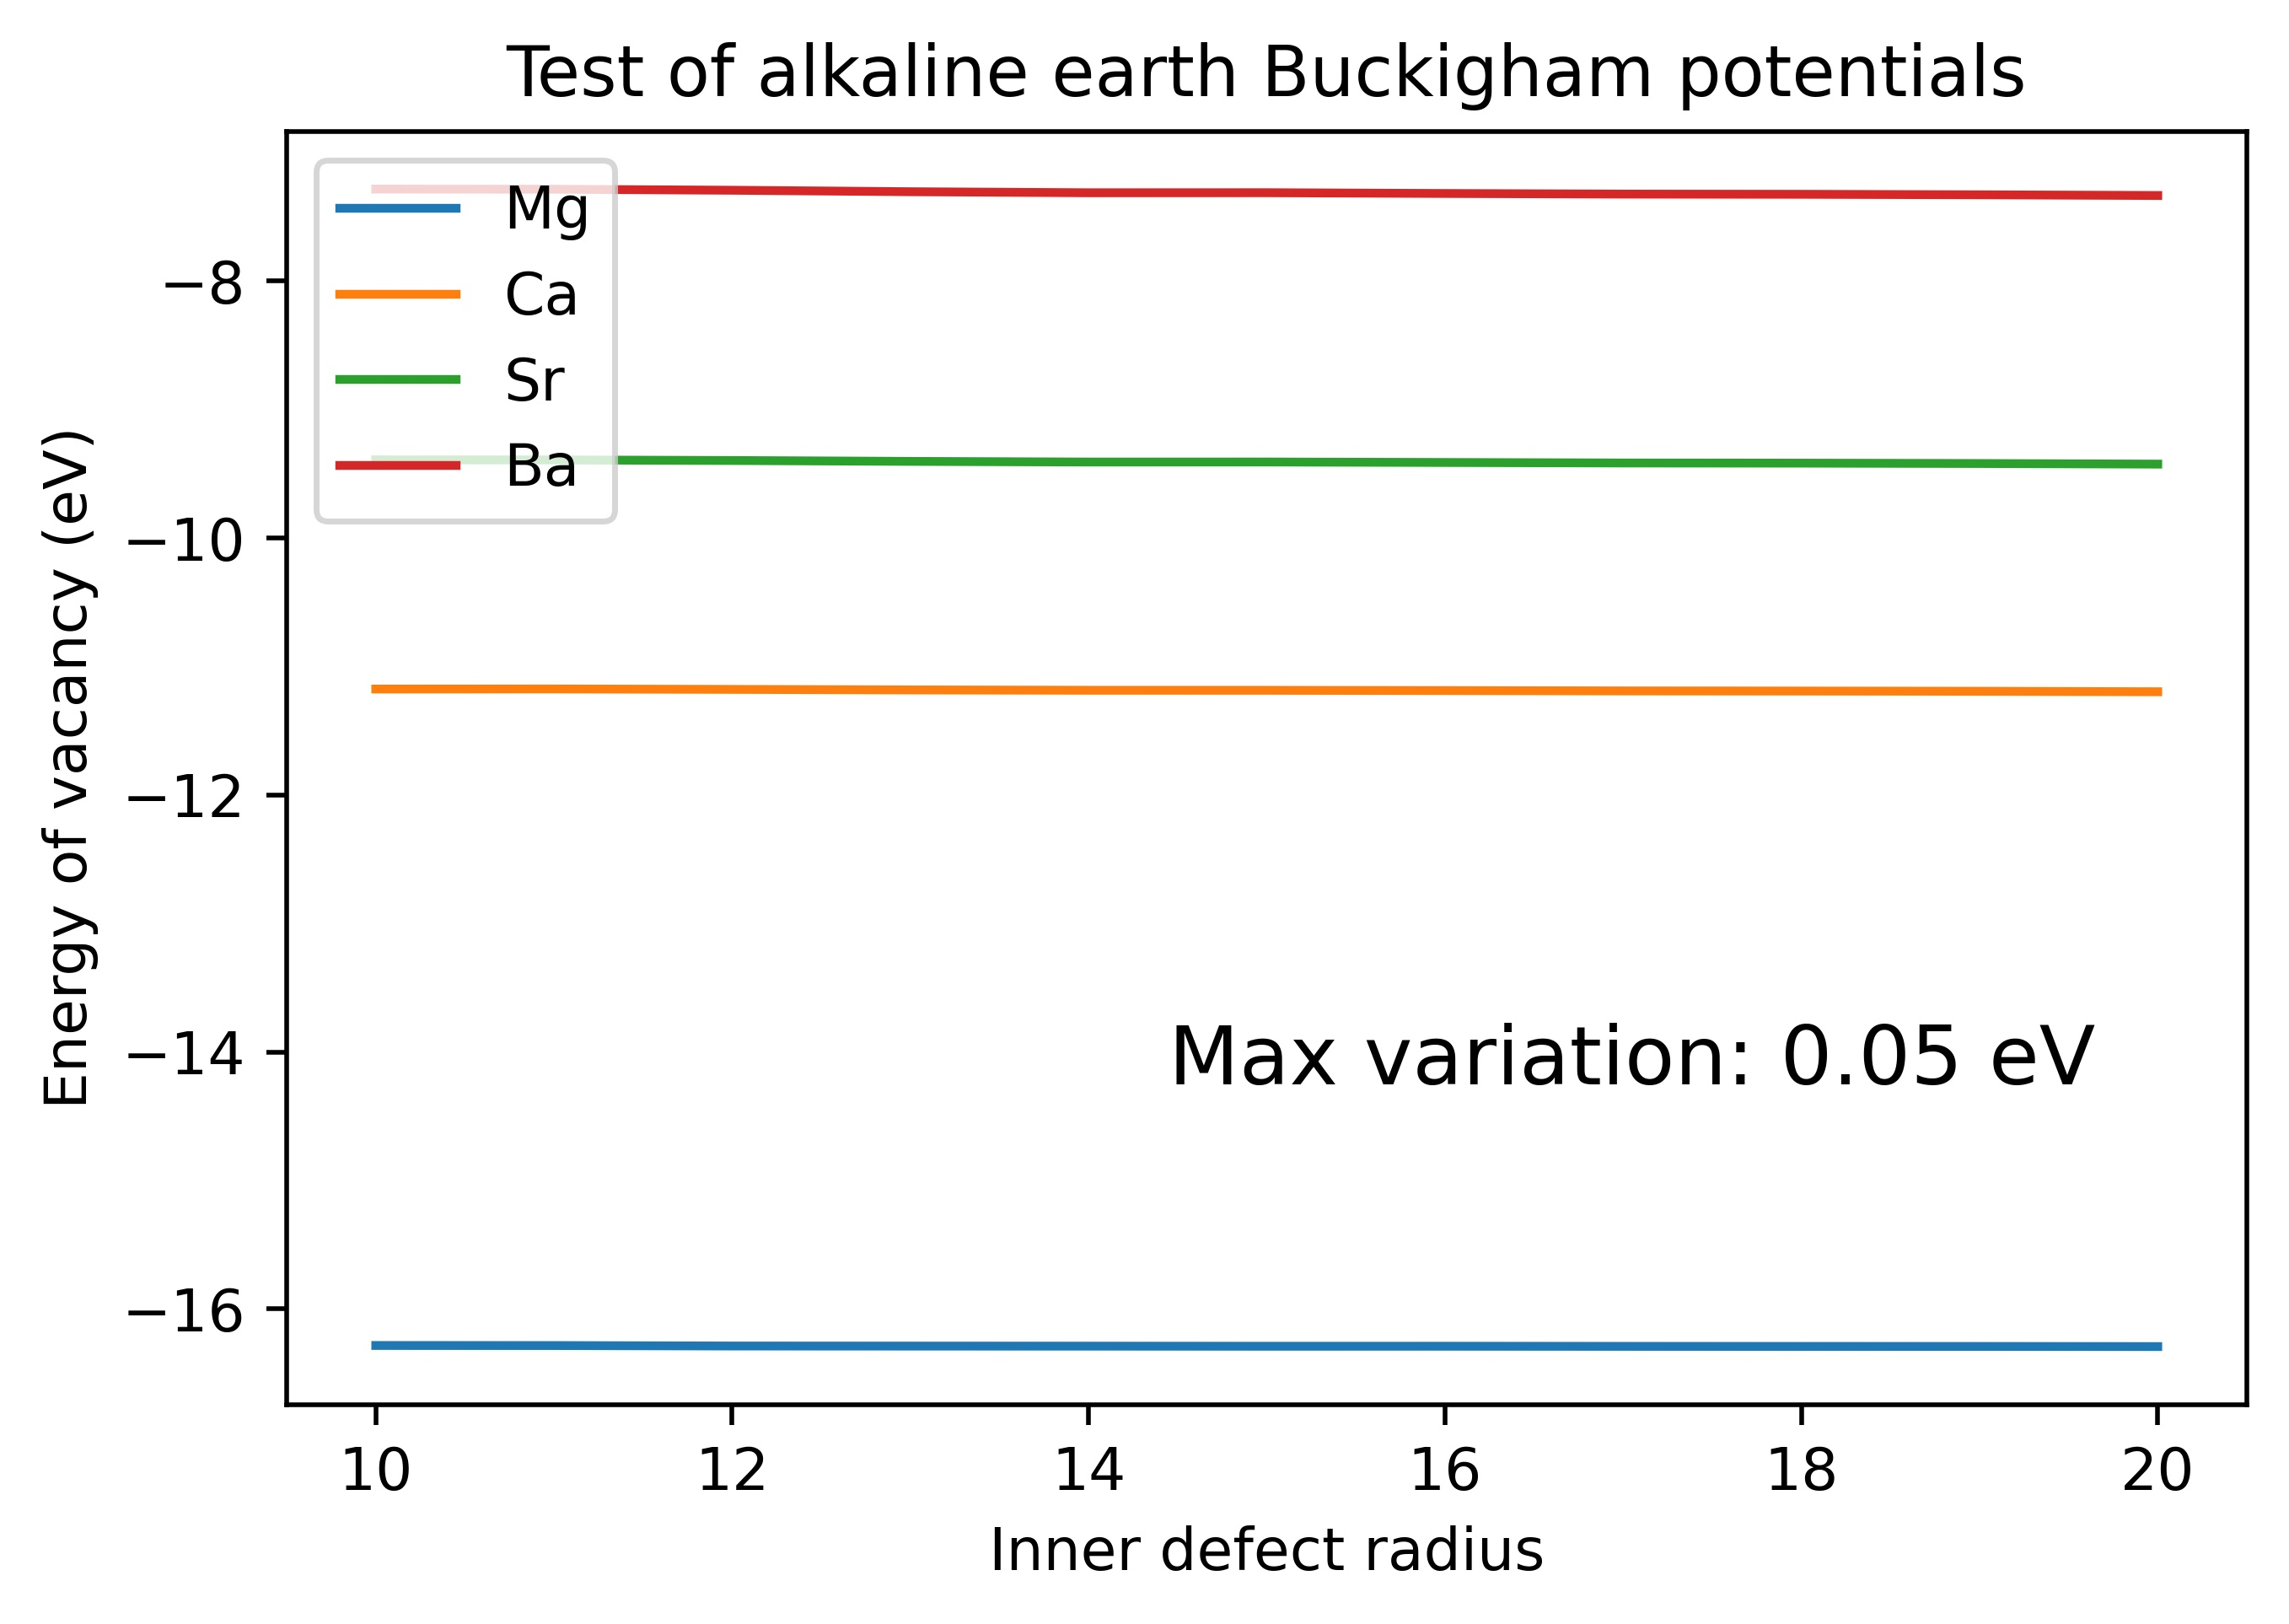
\includegraphics[width=0.75\textwidth]{buckingham_test.jpg}
\end{figure}

\end{frame}

\begin{frame}
\frametitle{The Effect of Calculation Setting on Energies}

\begin{figure}
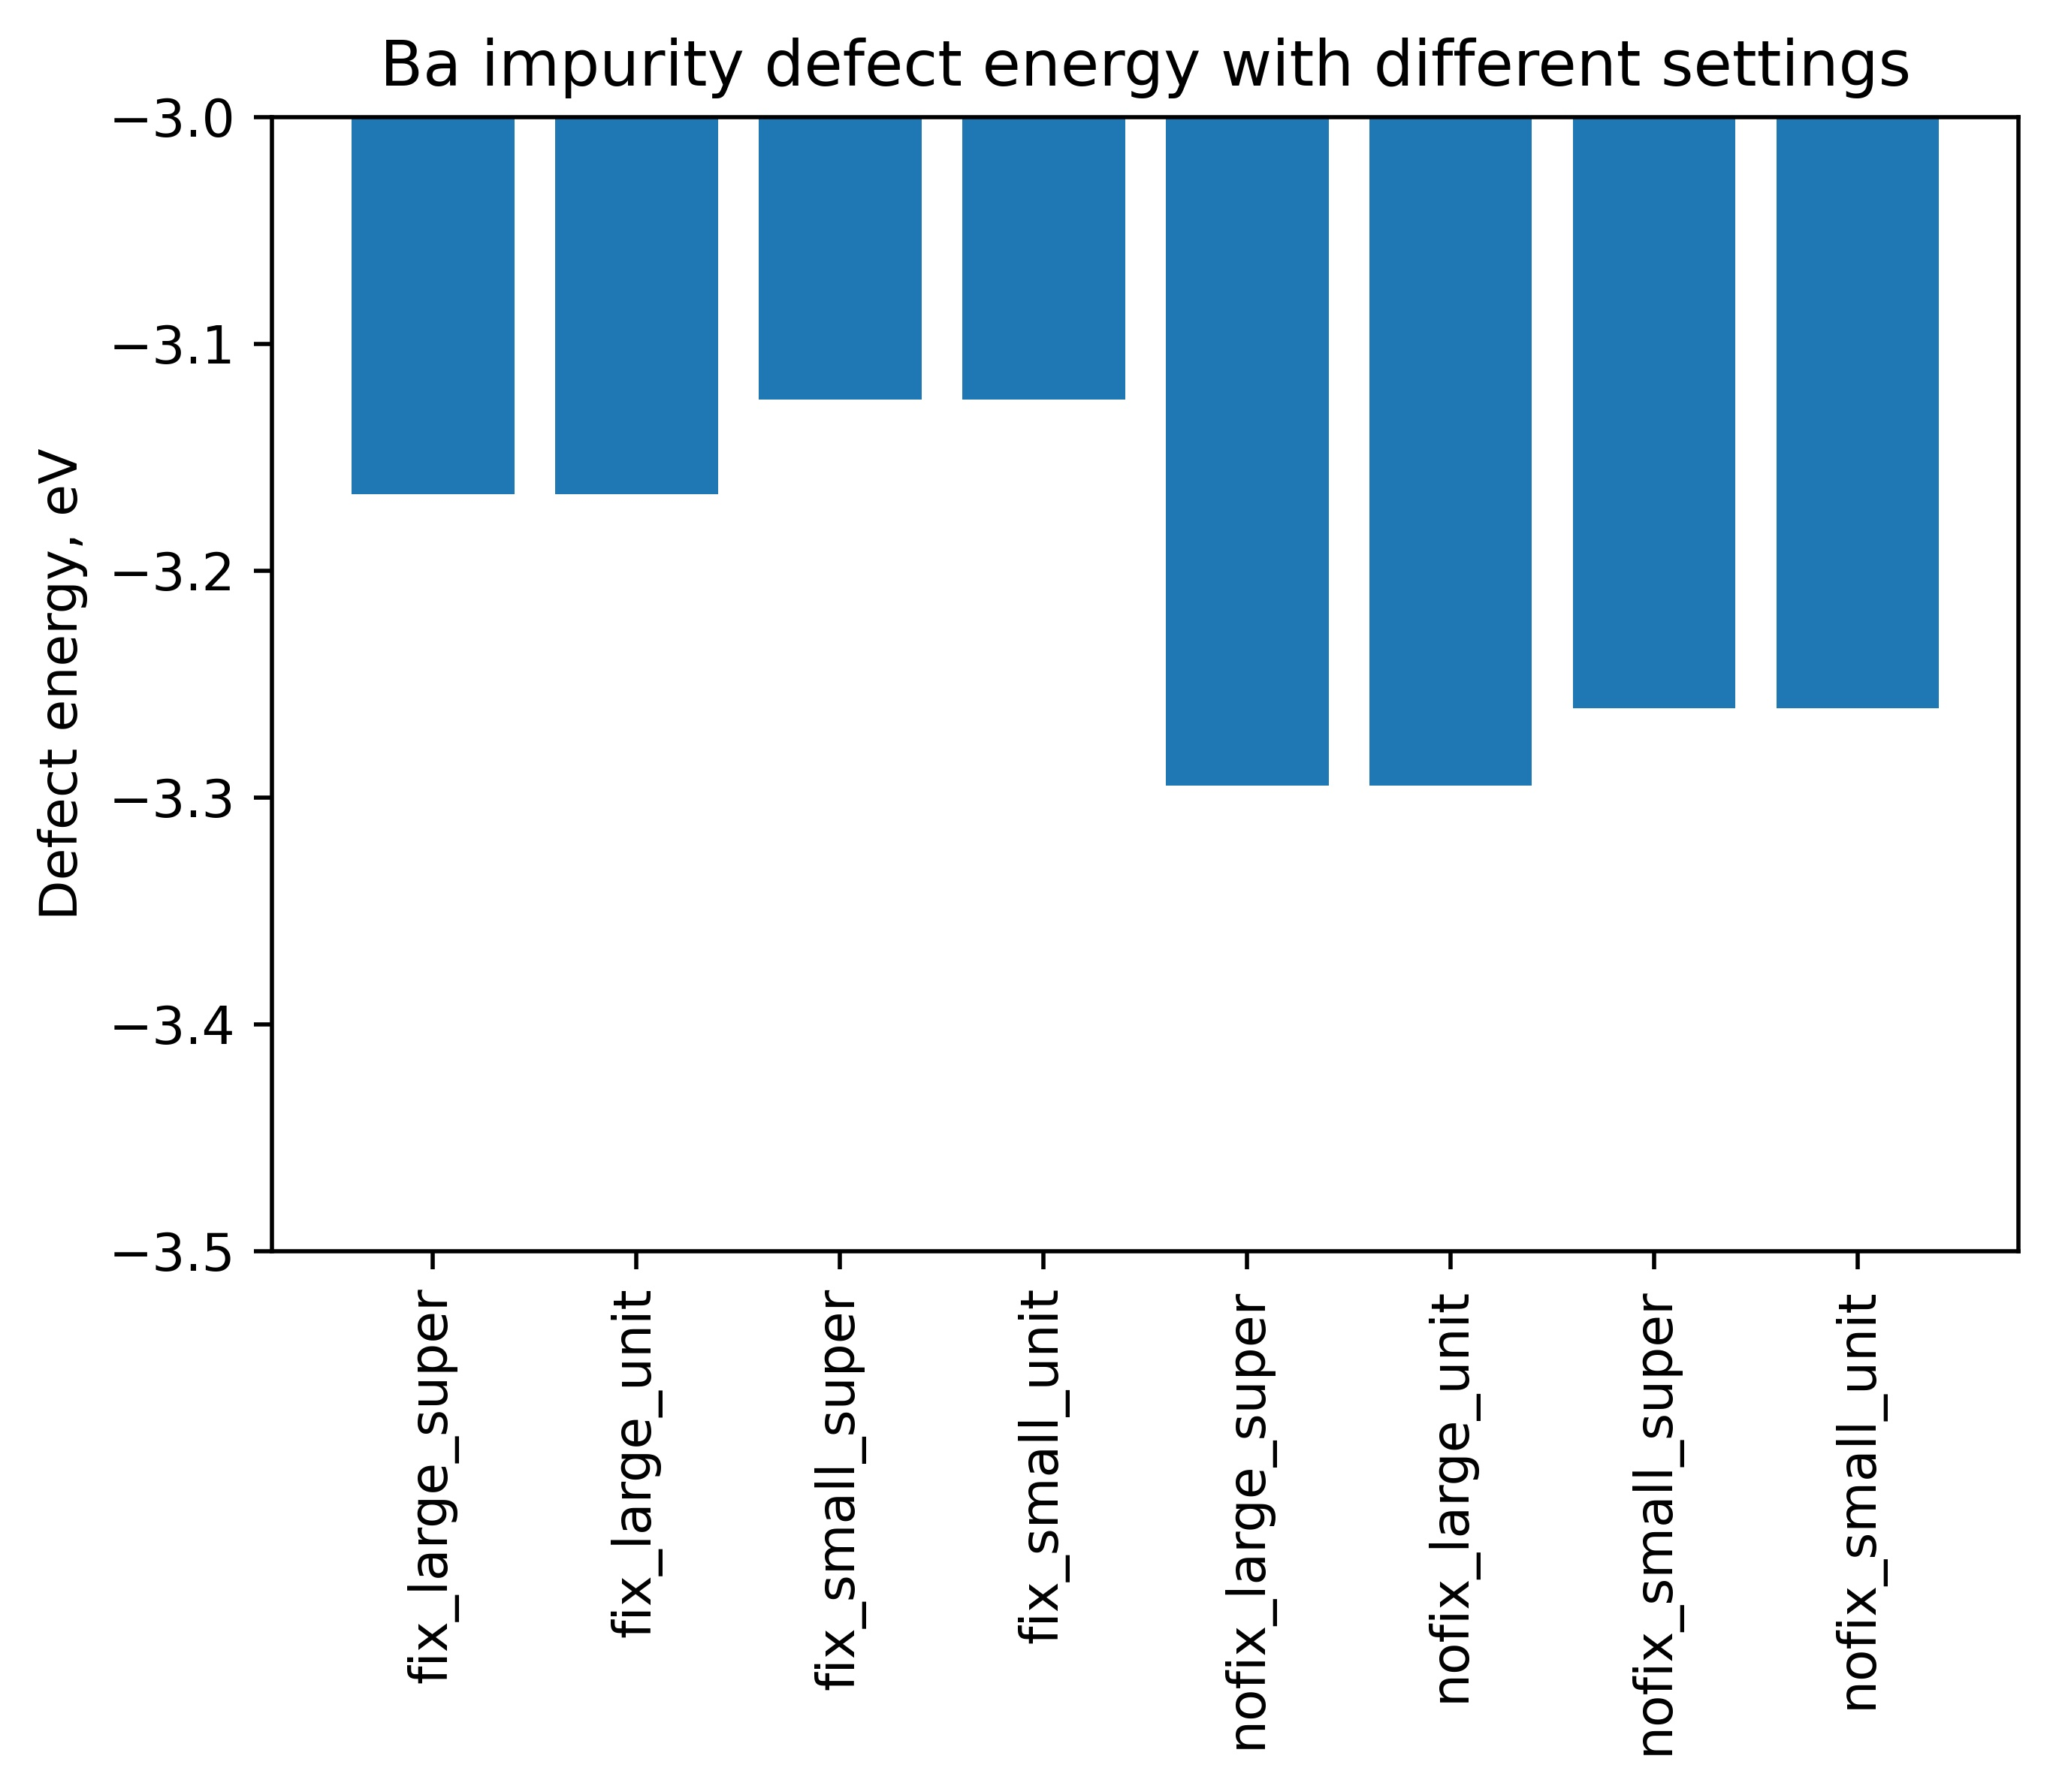
\includegraphics[width=0.75\textwidth]{energy_settings.jpg}
\end{figure}

\end{frame}

\begin{frame}
\frametitle{Lattice Energy Inconsistencies}

\begin{table}[h!]
  \begin{center}
  \resizebox{\textwidth}{!}{%
    \begin{tabular}{l|c|c|c}
      \textbf{Structure} & \textbf{Calculations} & \textbf{Calculations} & \textbf{Wan2018} \\
      & eV per unit cell & eV per formula unit & eV per formula unit \\
      \hline
      NaCl & -8.01 & -2.00 & NONE \\
      \ch{Na2O} & -26.38 & -6.60 & -11.3 \\
      MgO & -41.16 & -10.29 & -12.0 \\
      CaO & -35.88 & -8.97 & -12.9 \\
      SrO & -33.40 & -8.35 & -12.1 \\
      BaO & -31.20 & -7.80 & -11.6 \\      
    \end{tabular}}
  \end{center}
\end{table}

\end{frame}

\begin{frame}
\frametitle{NaCl Schottky Configurations}

\begin{figure}
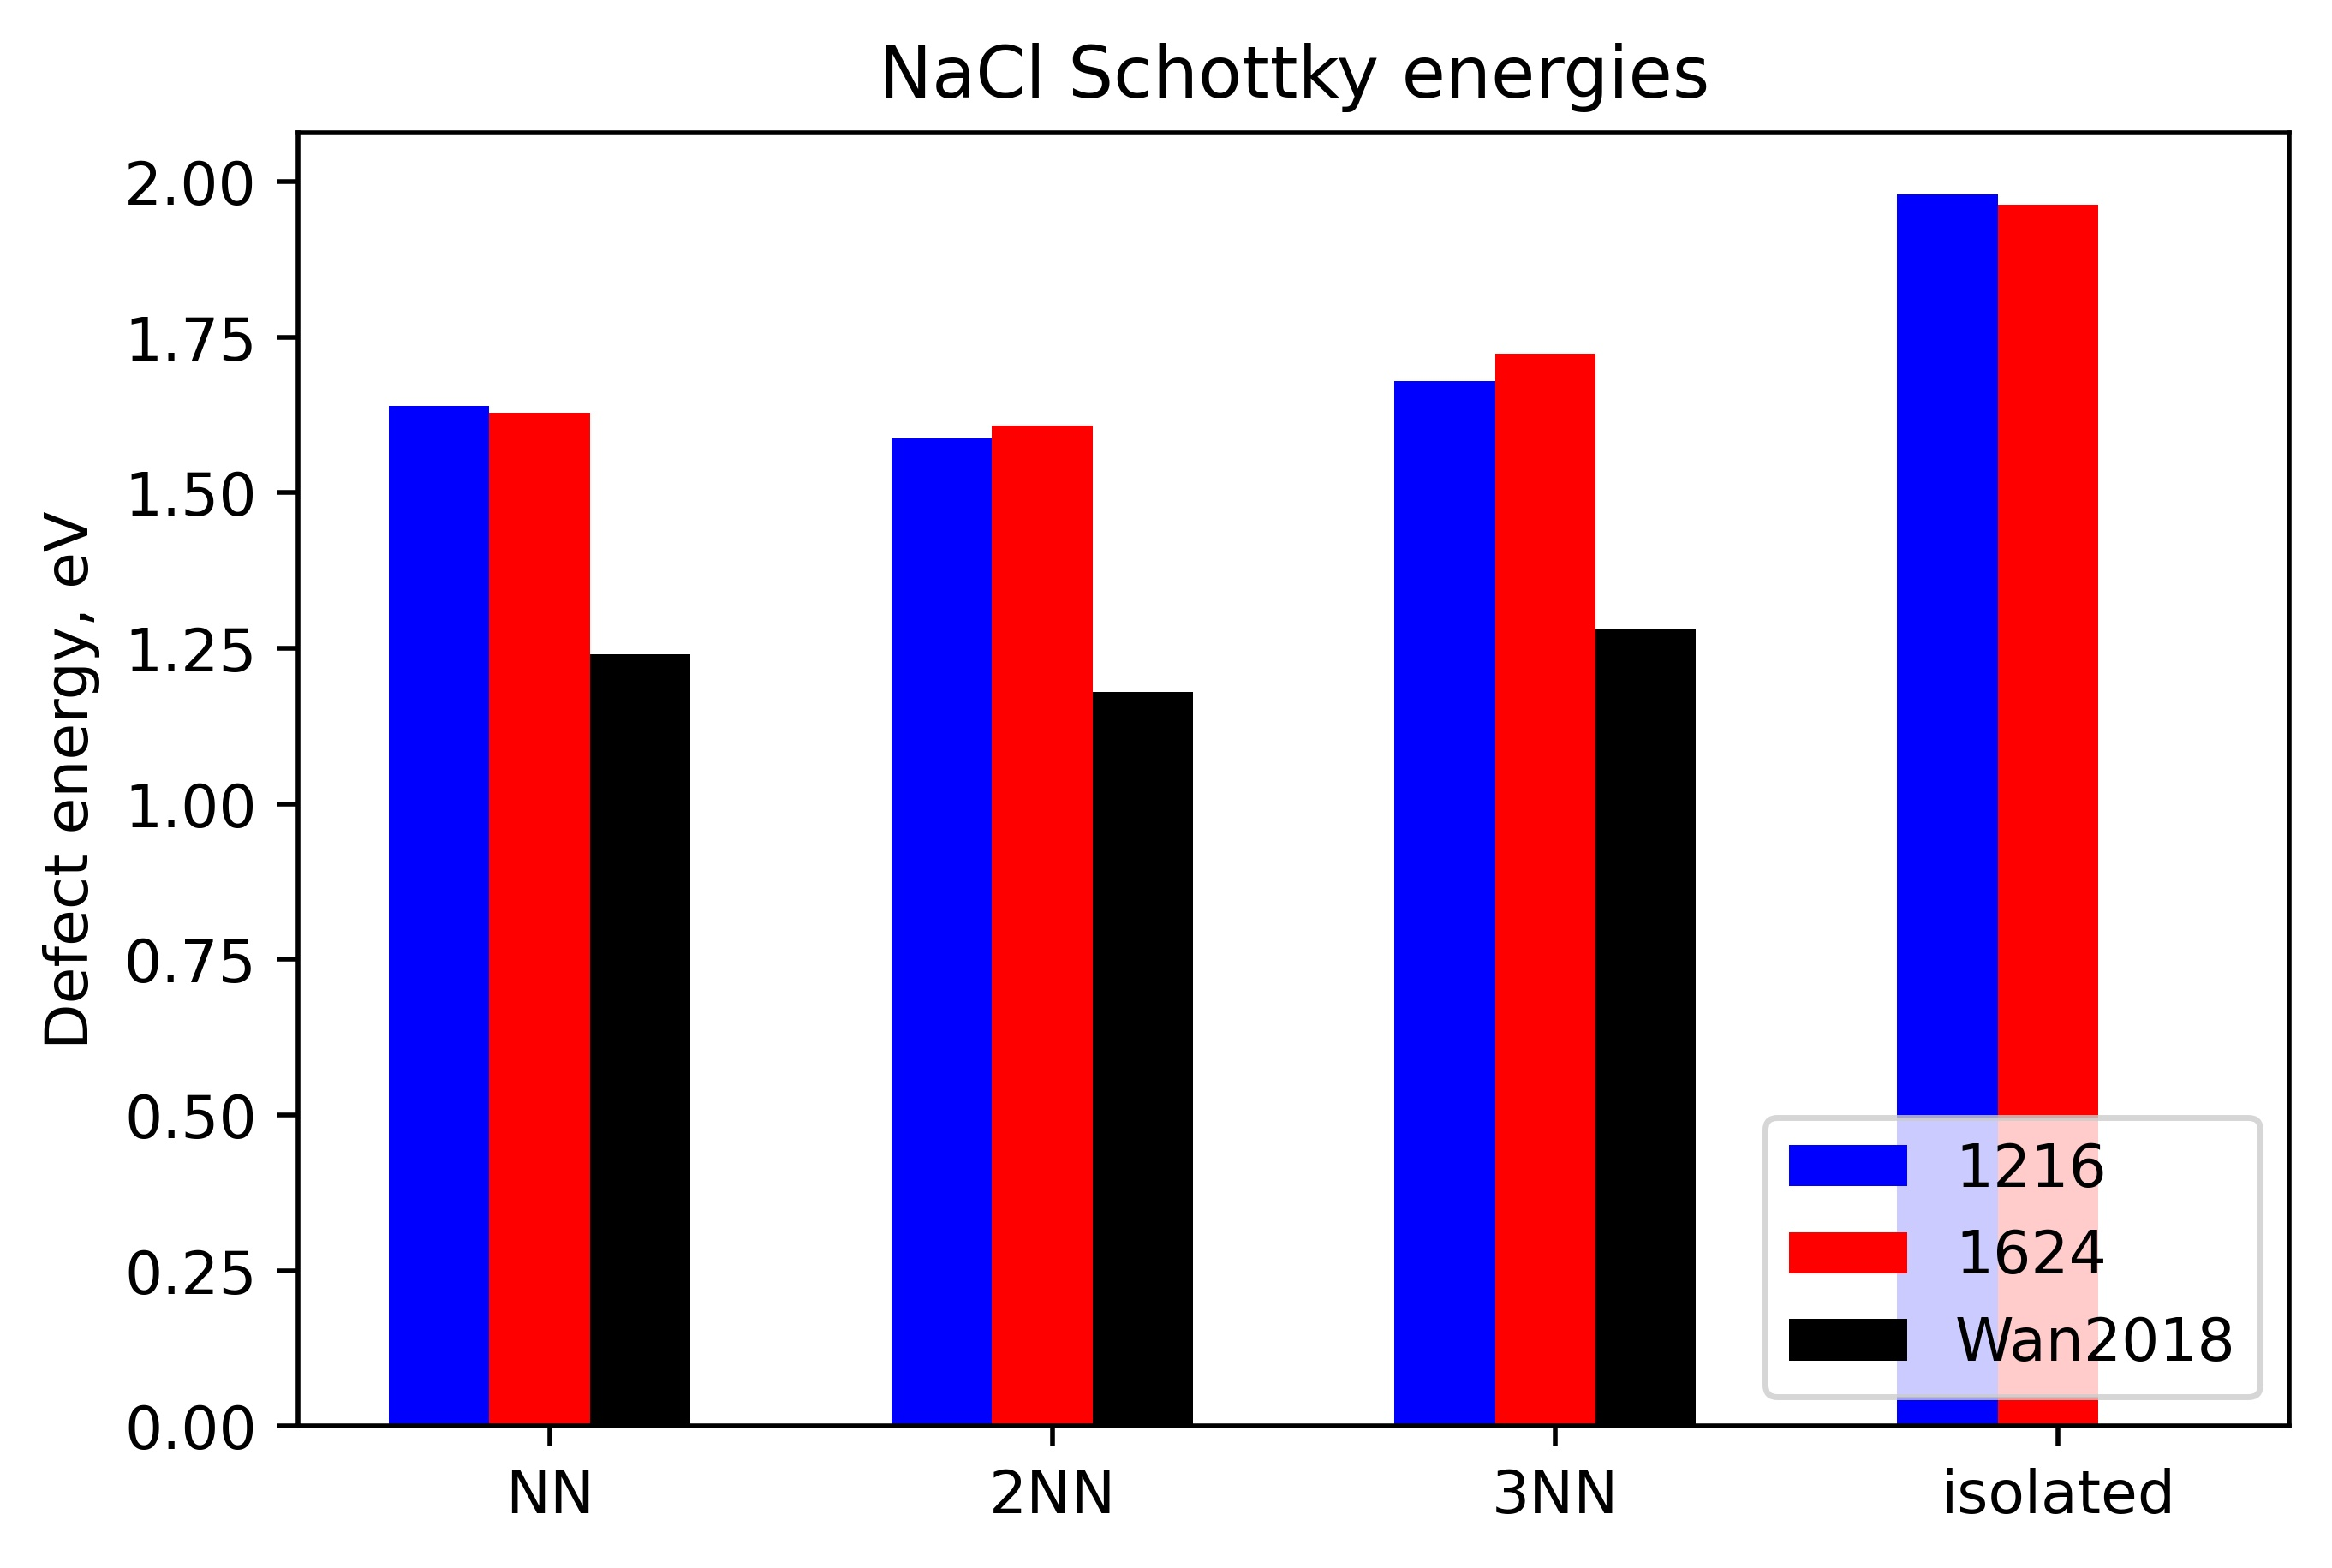
\includegraphics[width=0.4\textwidth]{schottky_nacl_absolute.jpg}
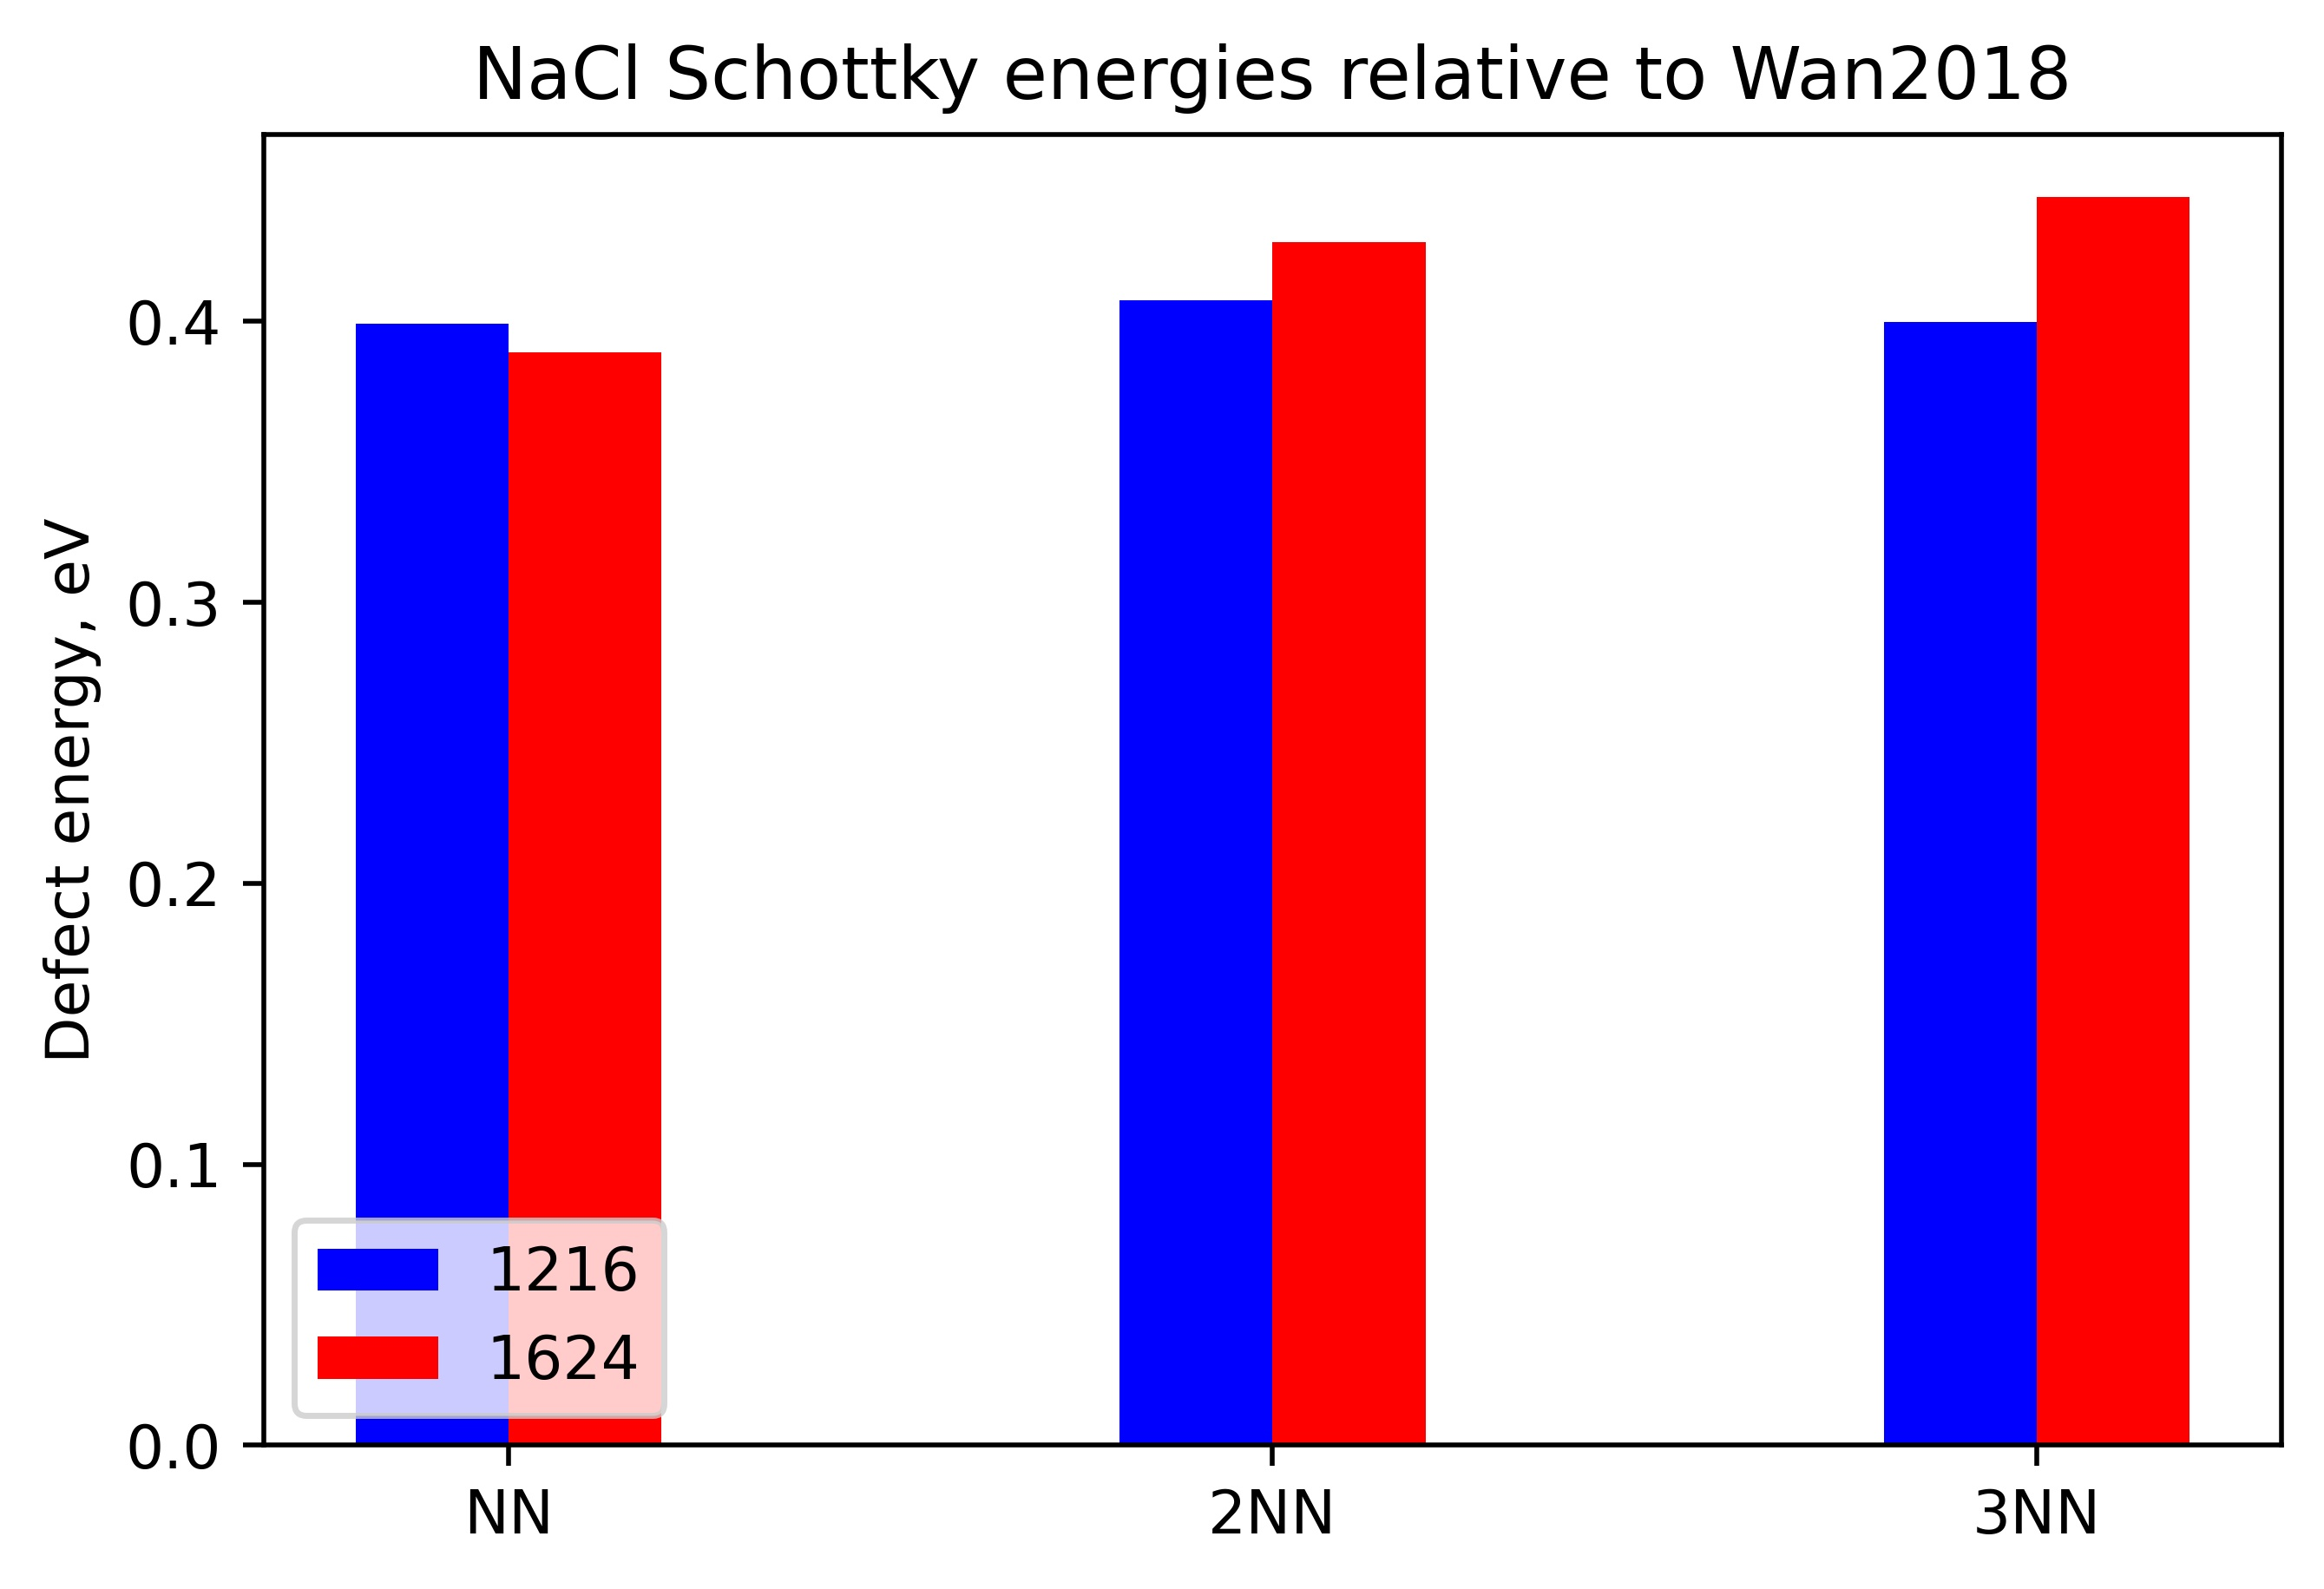
\includegraphics[width=0.4\textwidth]{schottky_nacl_relative.jpg}
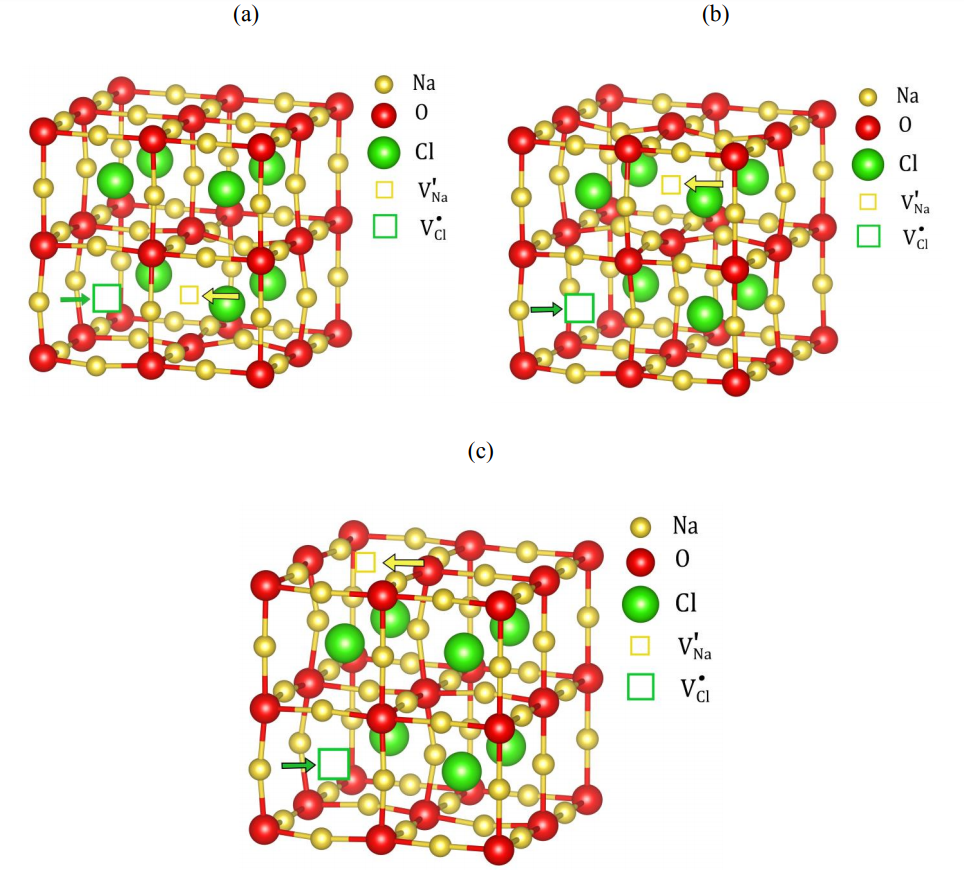
\includegraphics[width=0.5\textwidth]{defect_configs.png}
\end{figure}

\end{frame}

\begin{frame}
\frametitle{\ch{Na2O} Schottky Configurations}

\begin{figure}
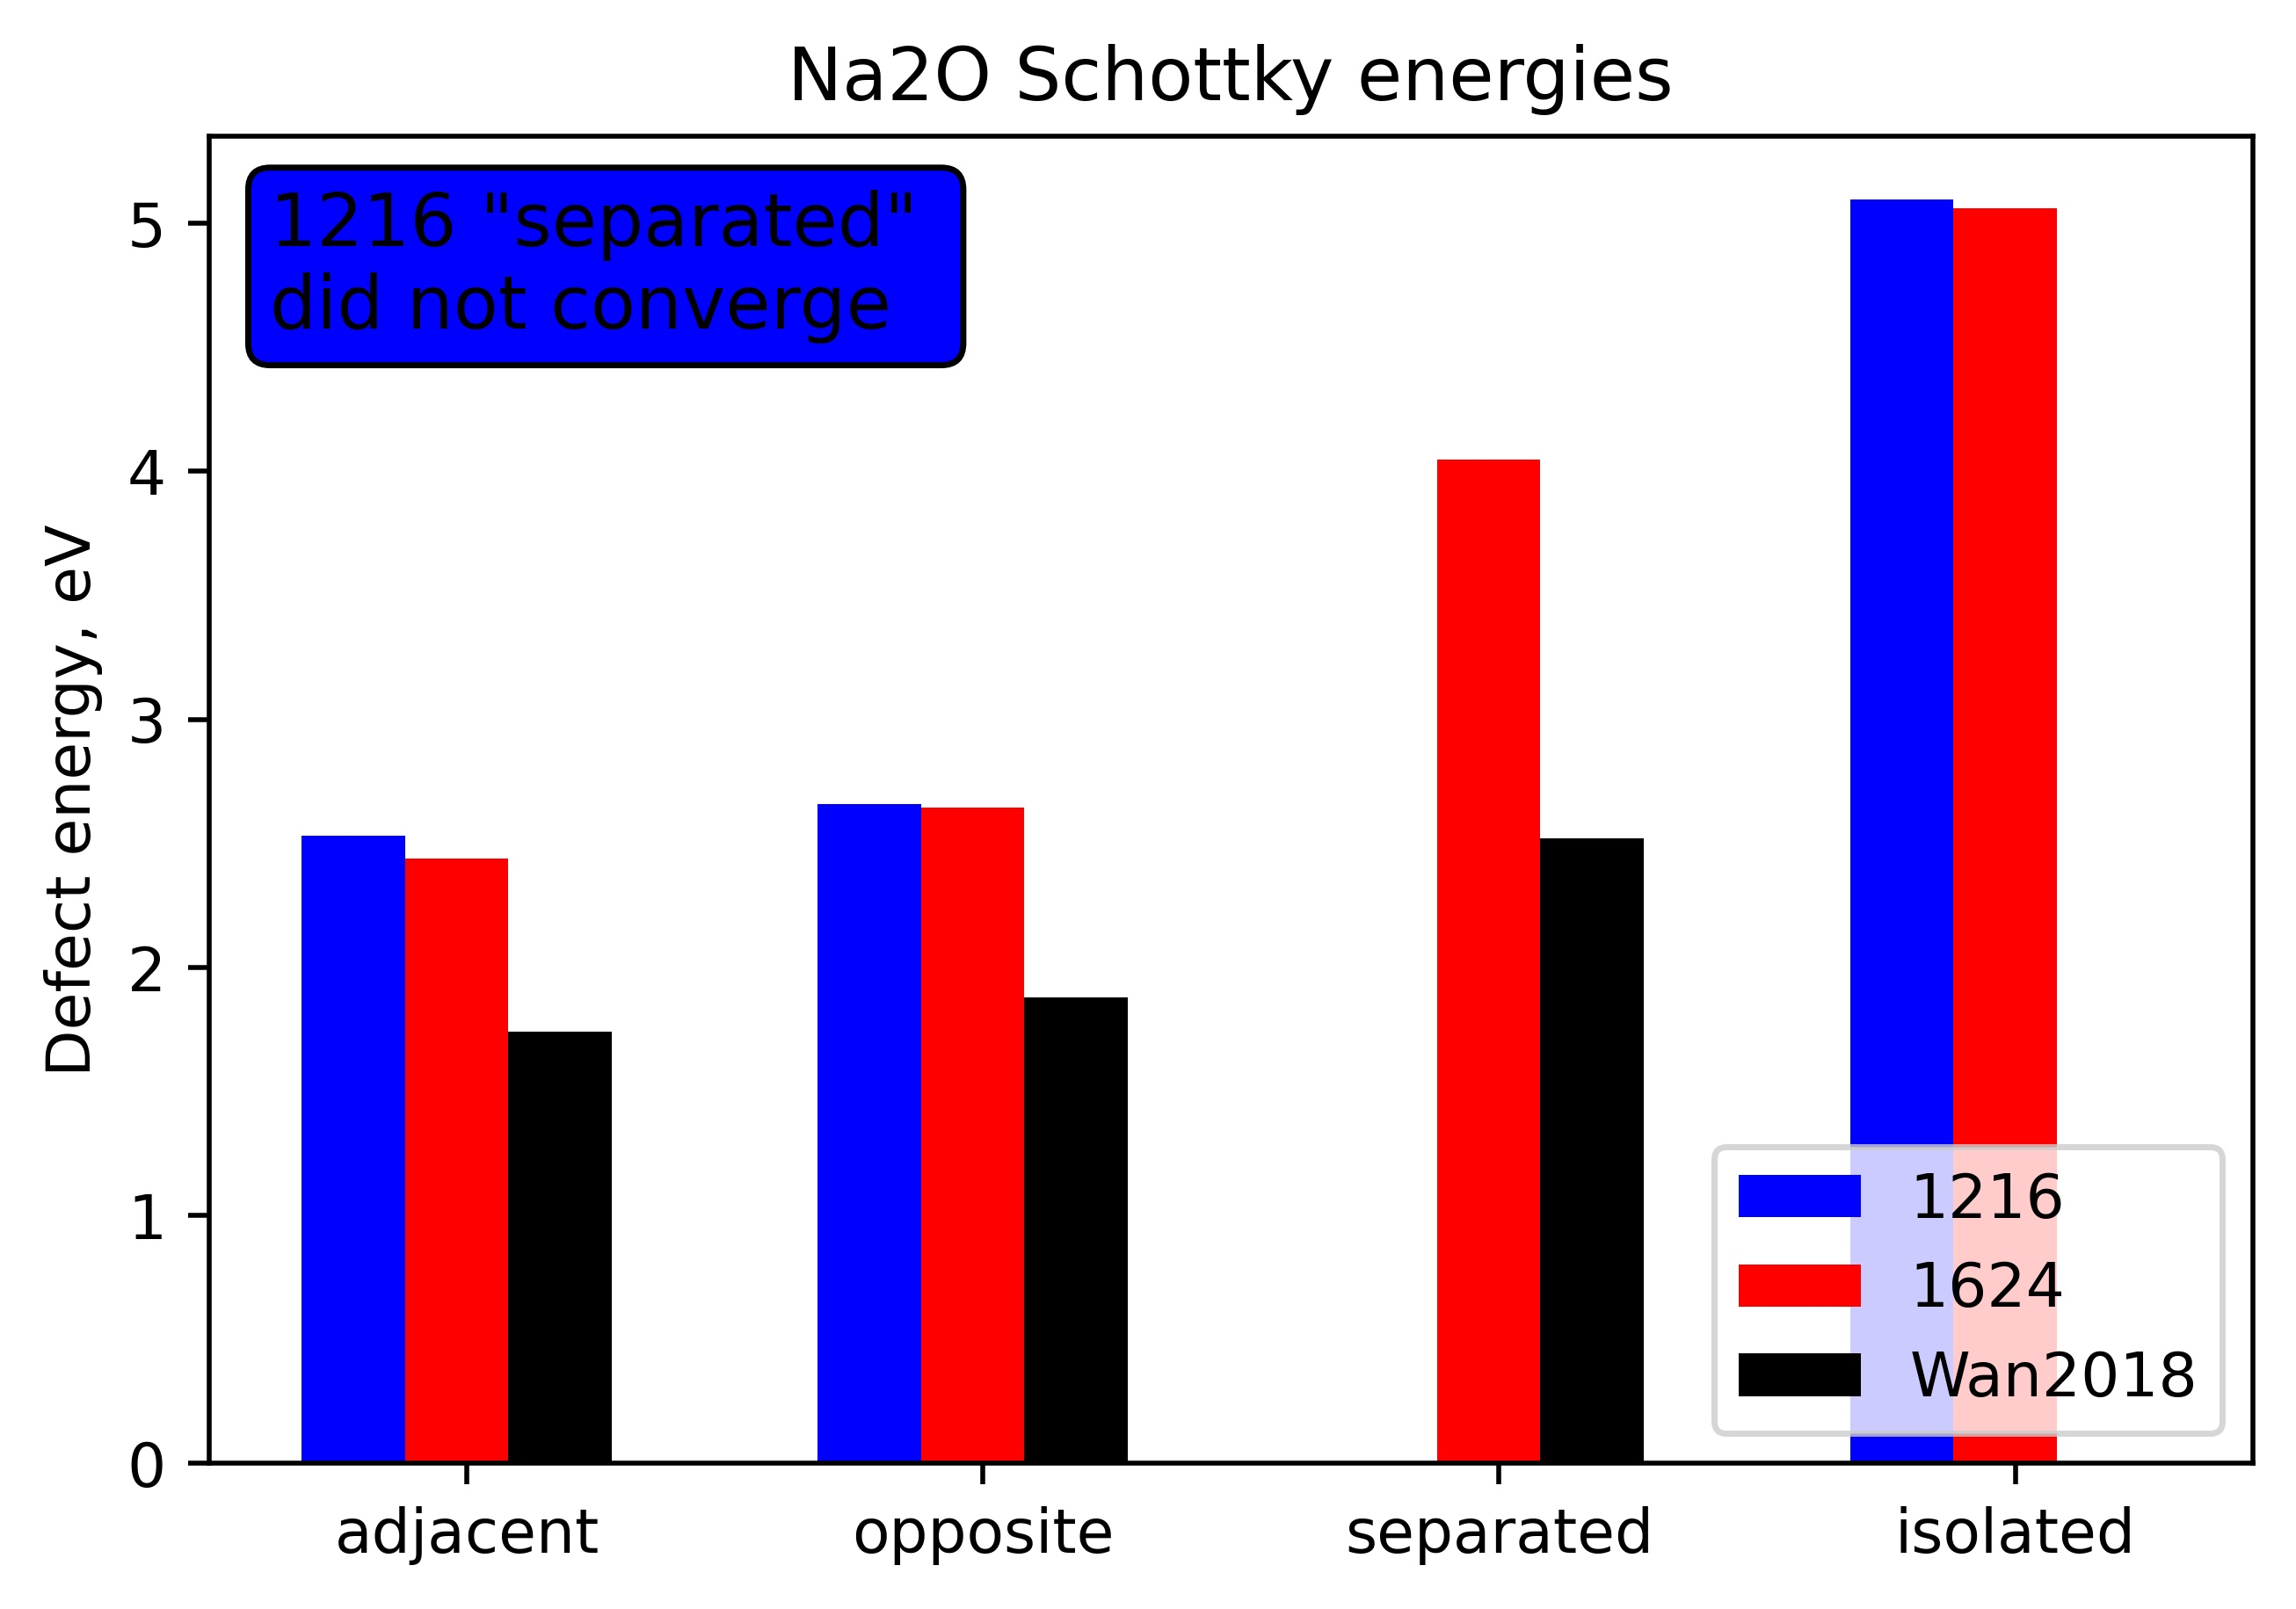
\includegraphics[width=0.4\textwidth]{schottky_na2o_absolute.jpg}
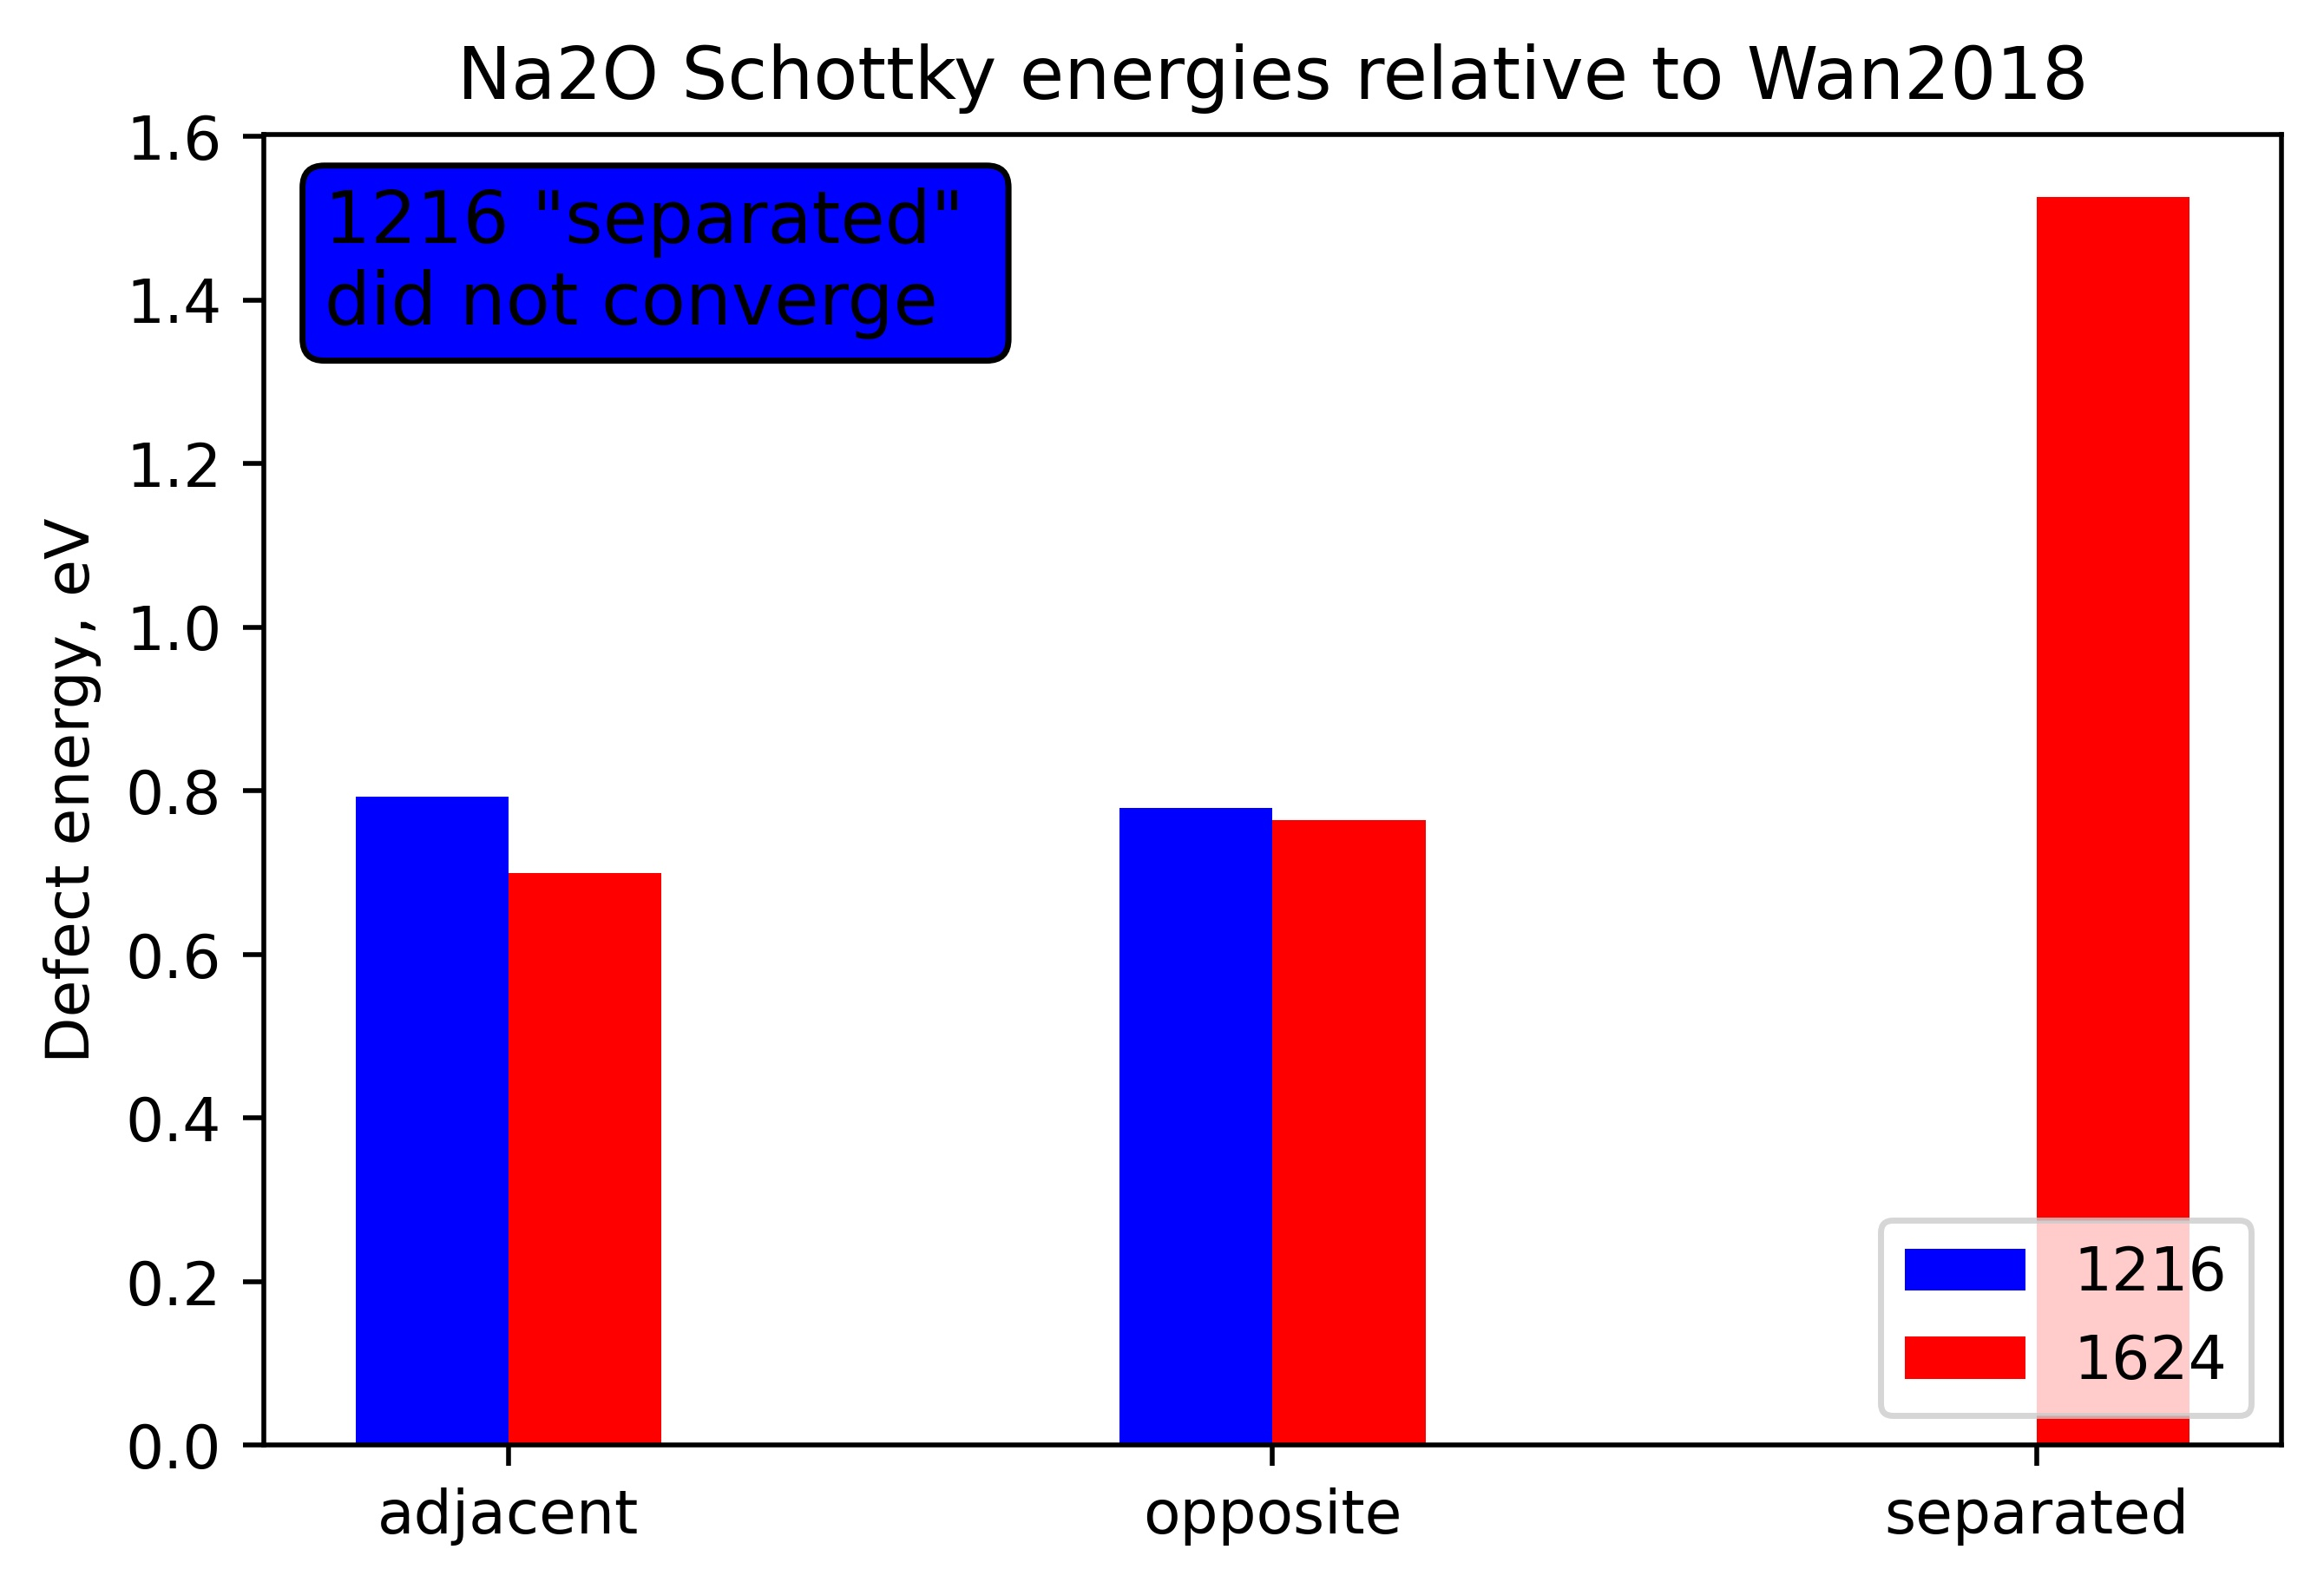
\includegraphics[width=0.4\textwidth]{schottky_na2o_relative.jpg}
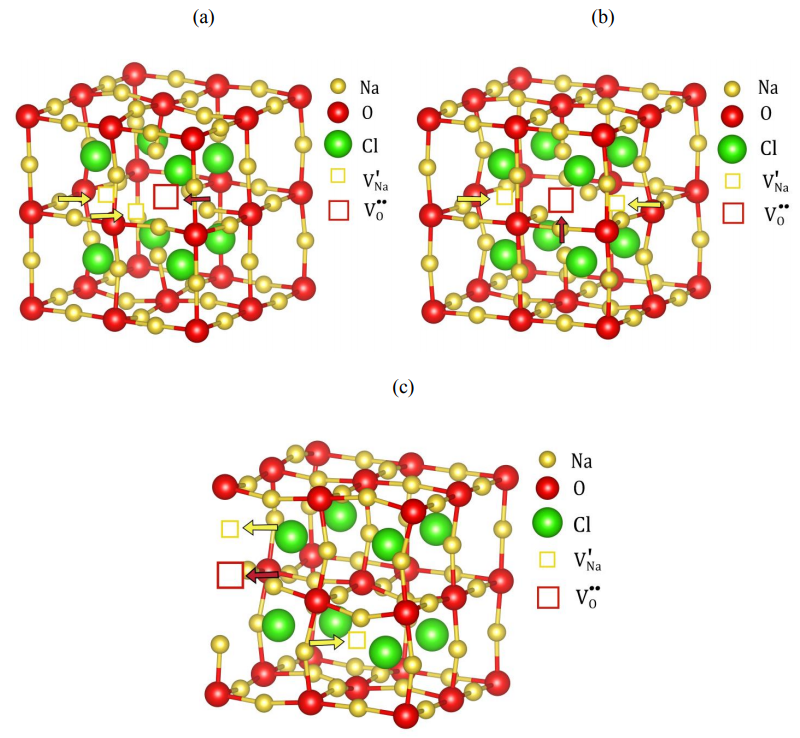
\includegraphics[width=0.5\textwidth]{na2o_configs.png}
\end{figure}

\end{frame}

\begin{frame}
\frametitle{Doping Configurations}

\begin{figure}
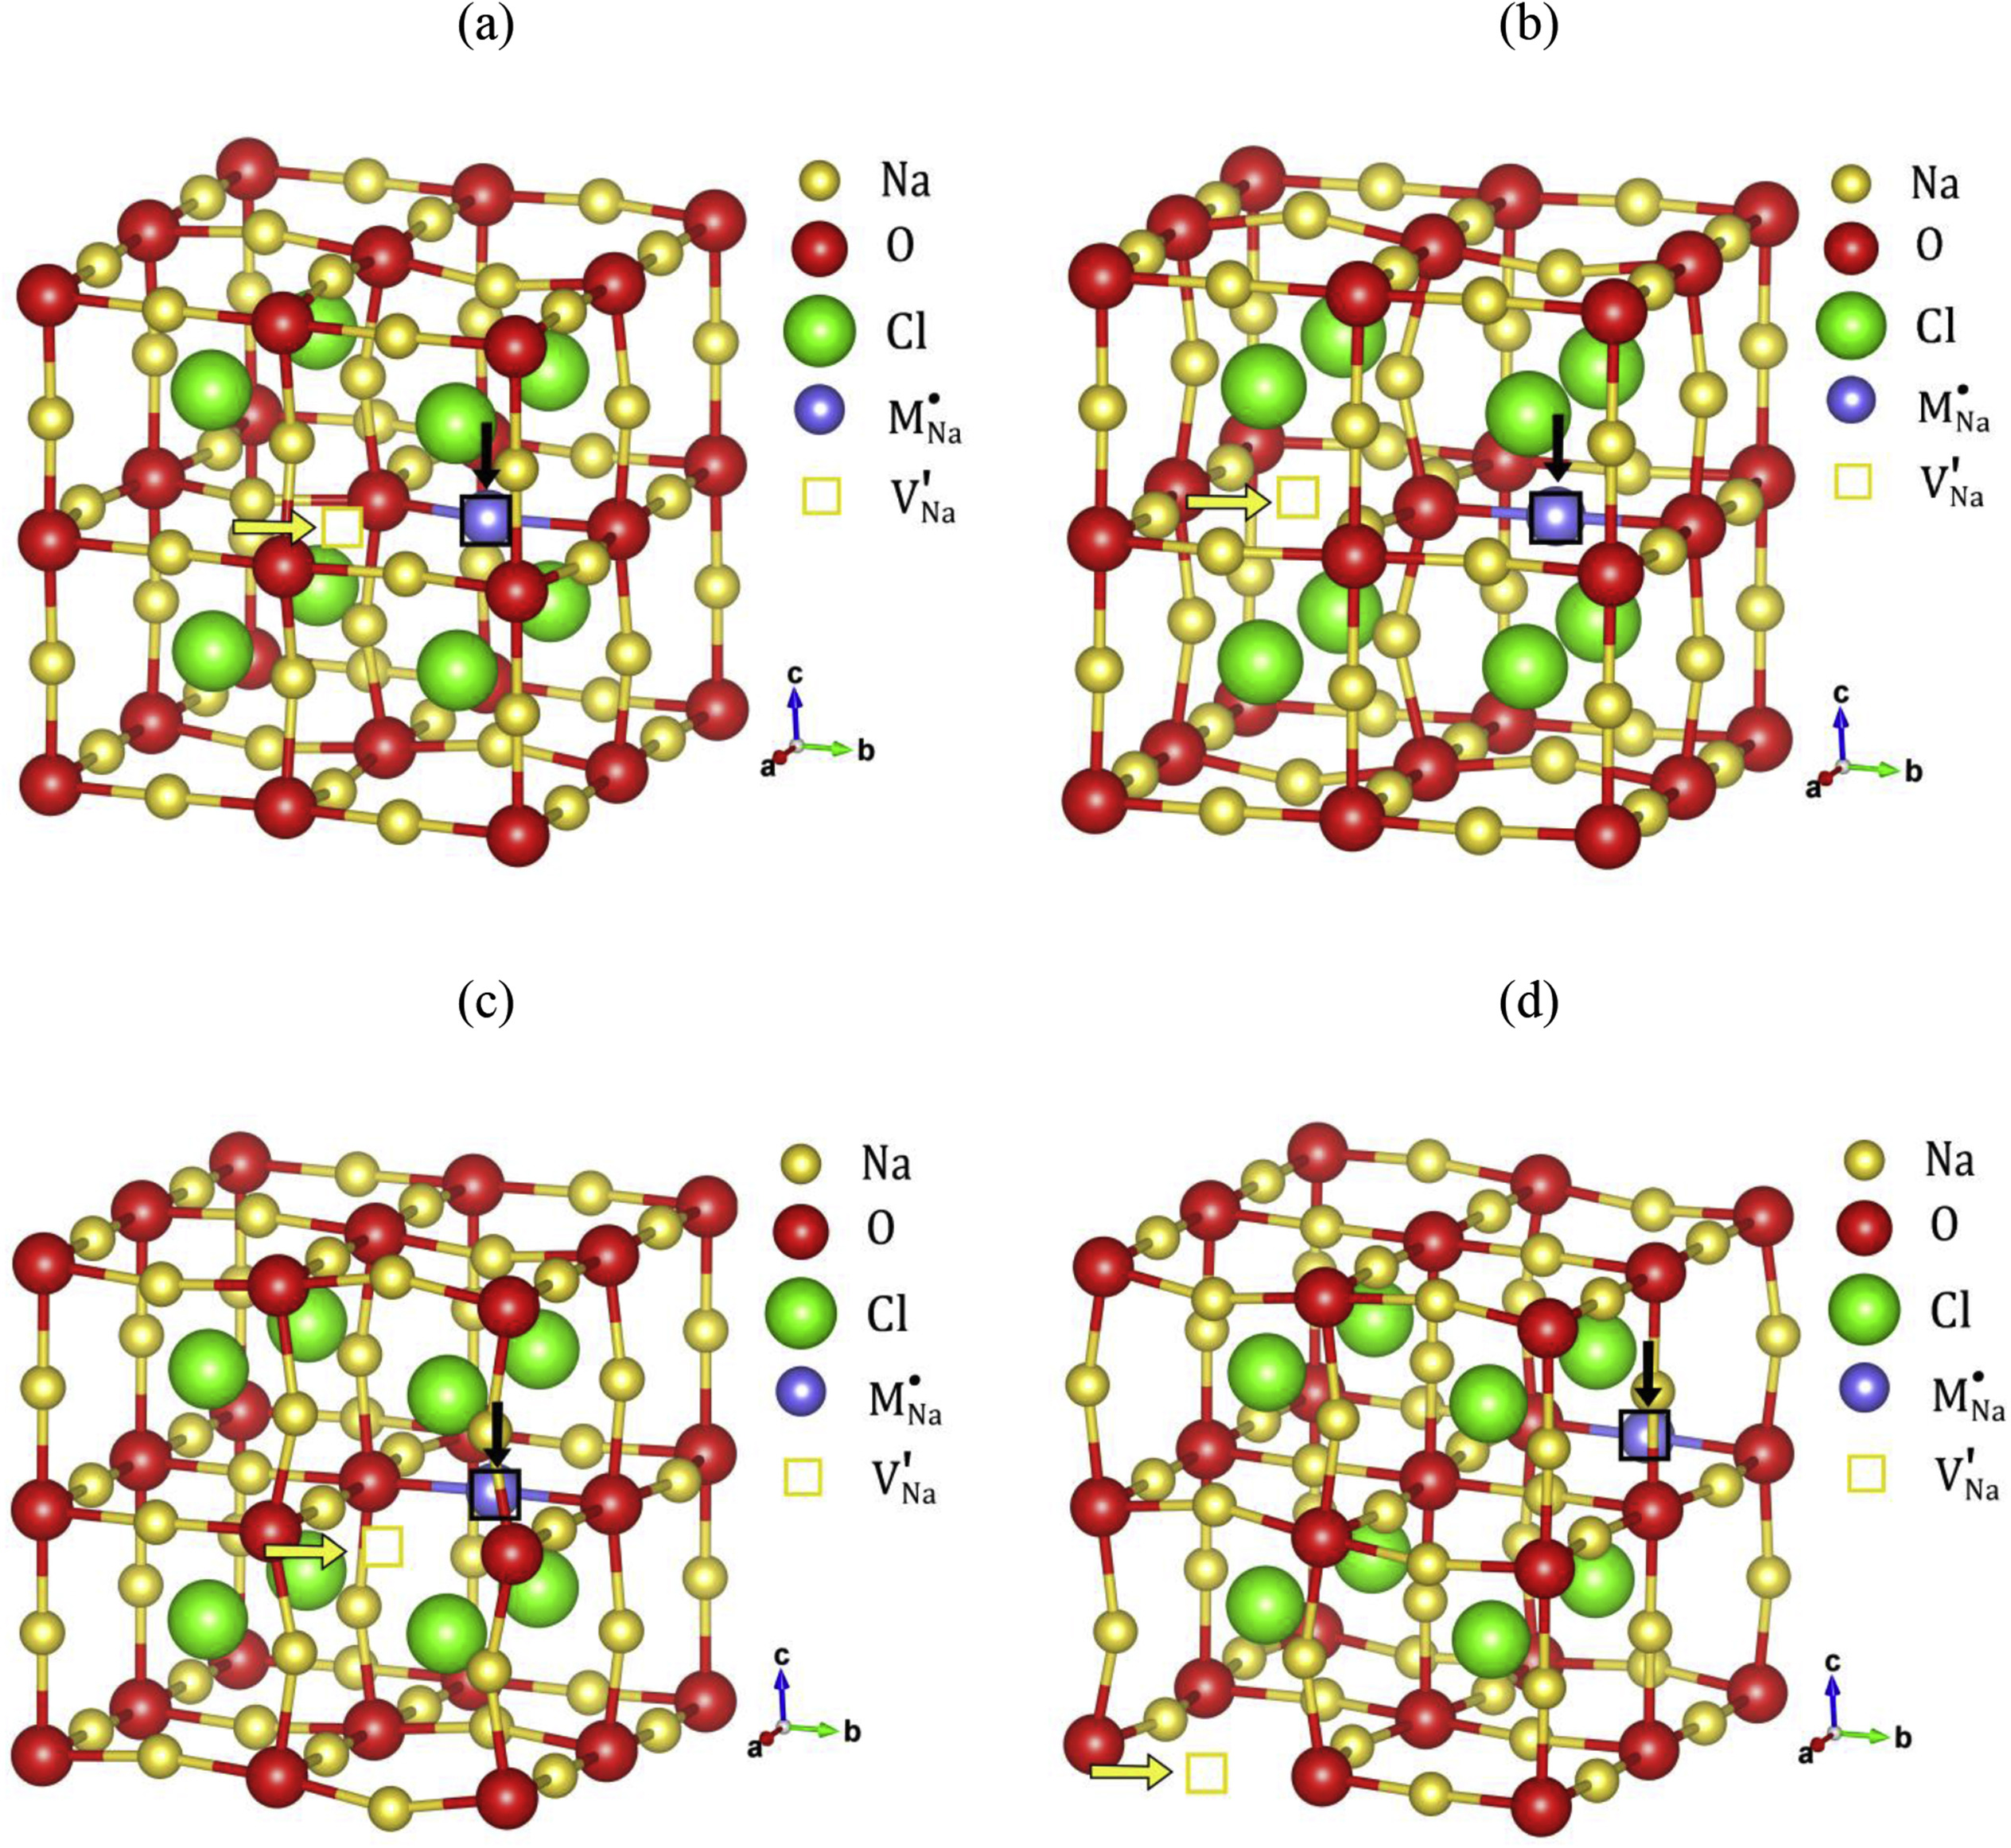
\includegraphics[width=0.75\textwidth]{doping_configs.jpg}
\end{figure}

\end{frame}

\begin{frame}
\frametitle{Doping Configurations}

\begin{figure}
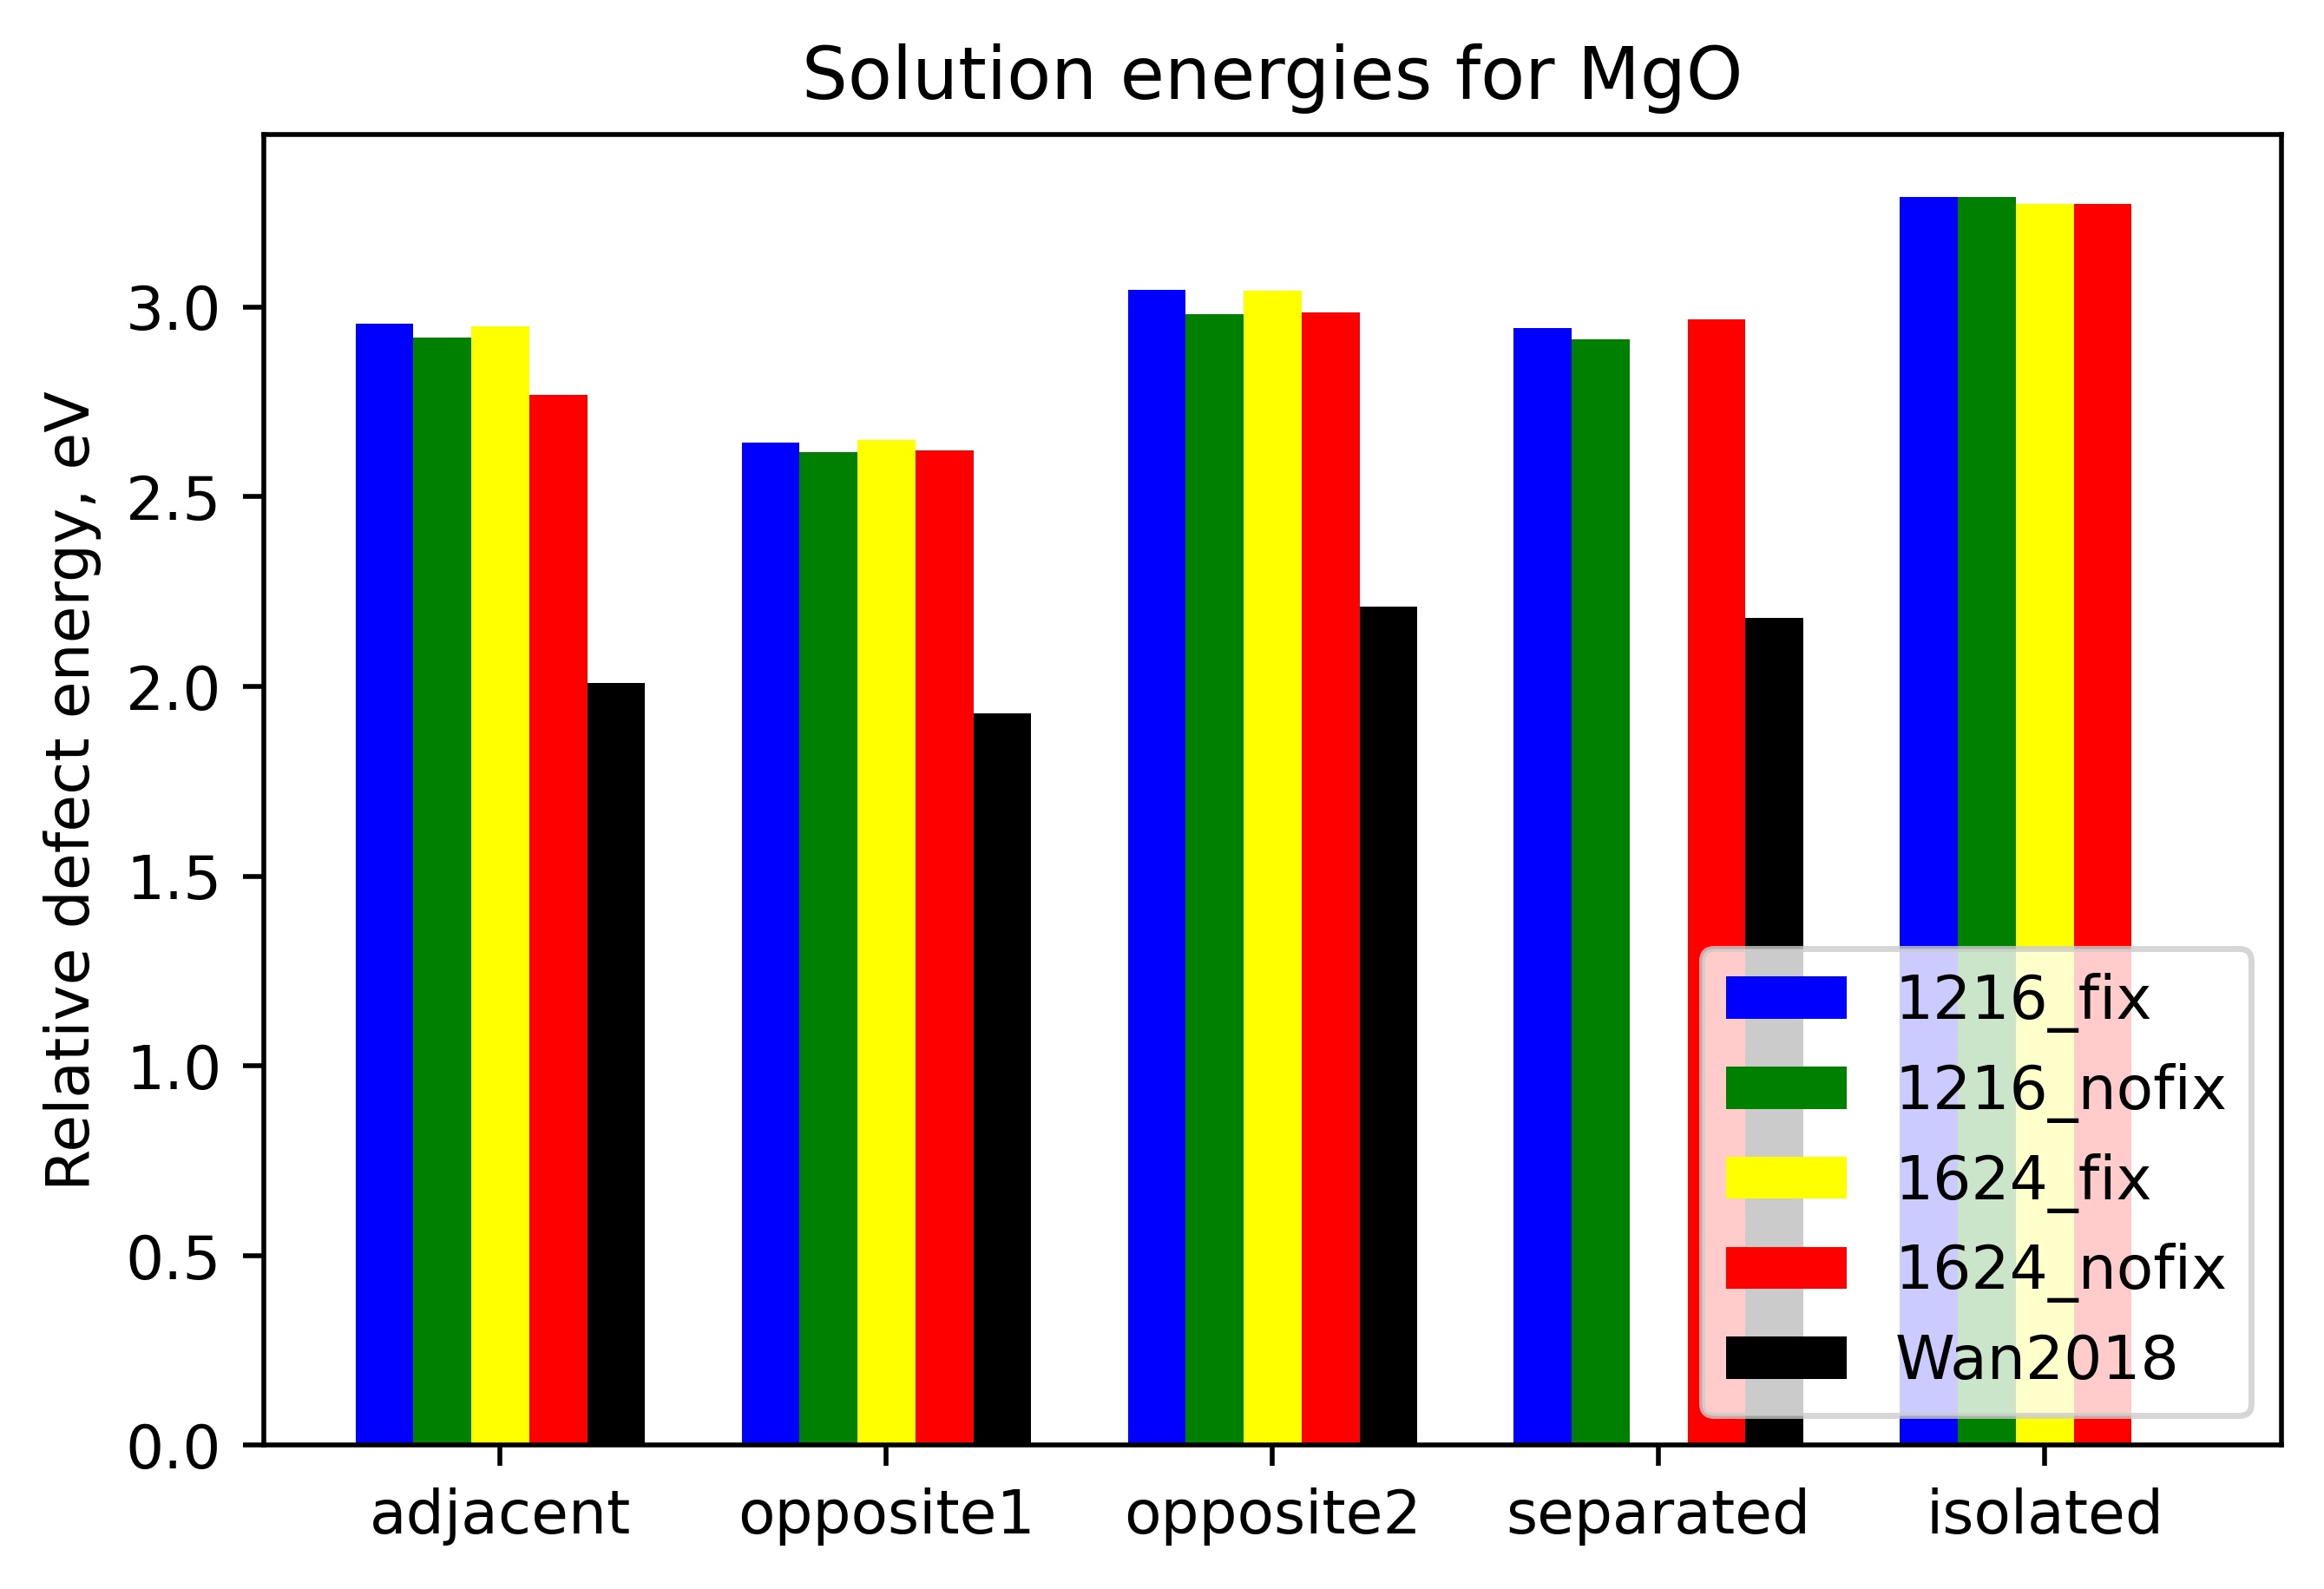
\includegraphics[width=0.4\textwidth]{mg_absolute.jpg}
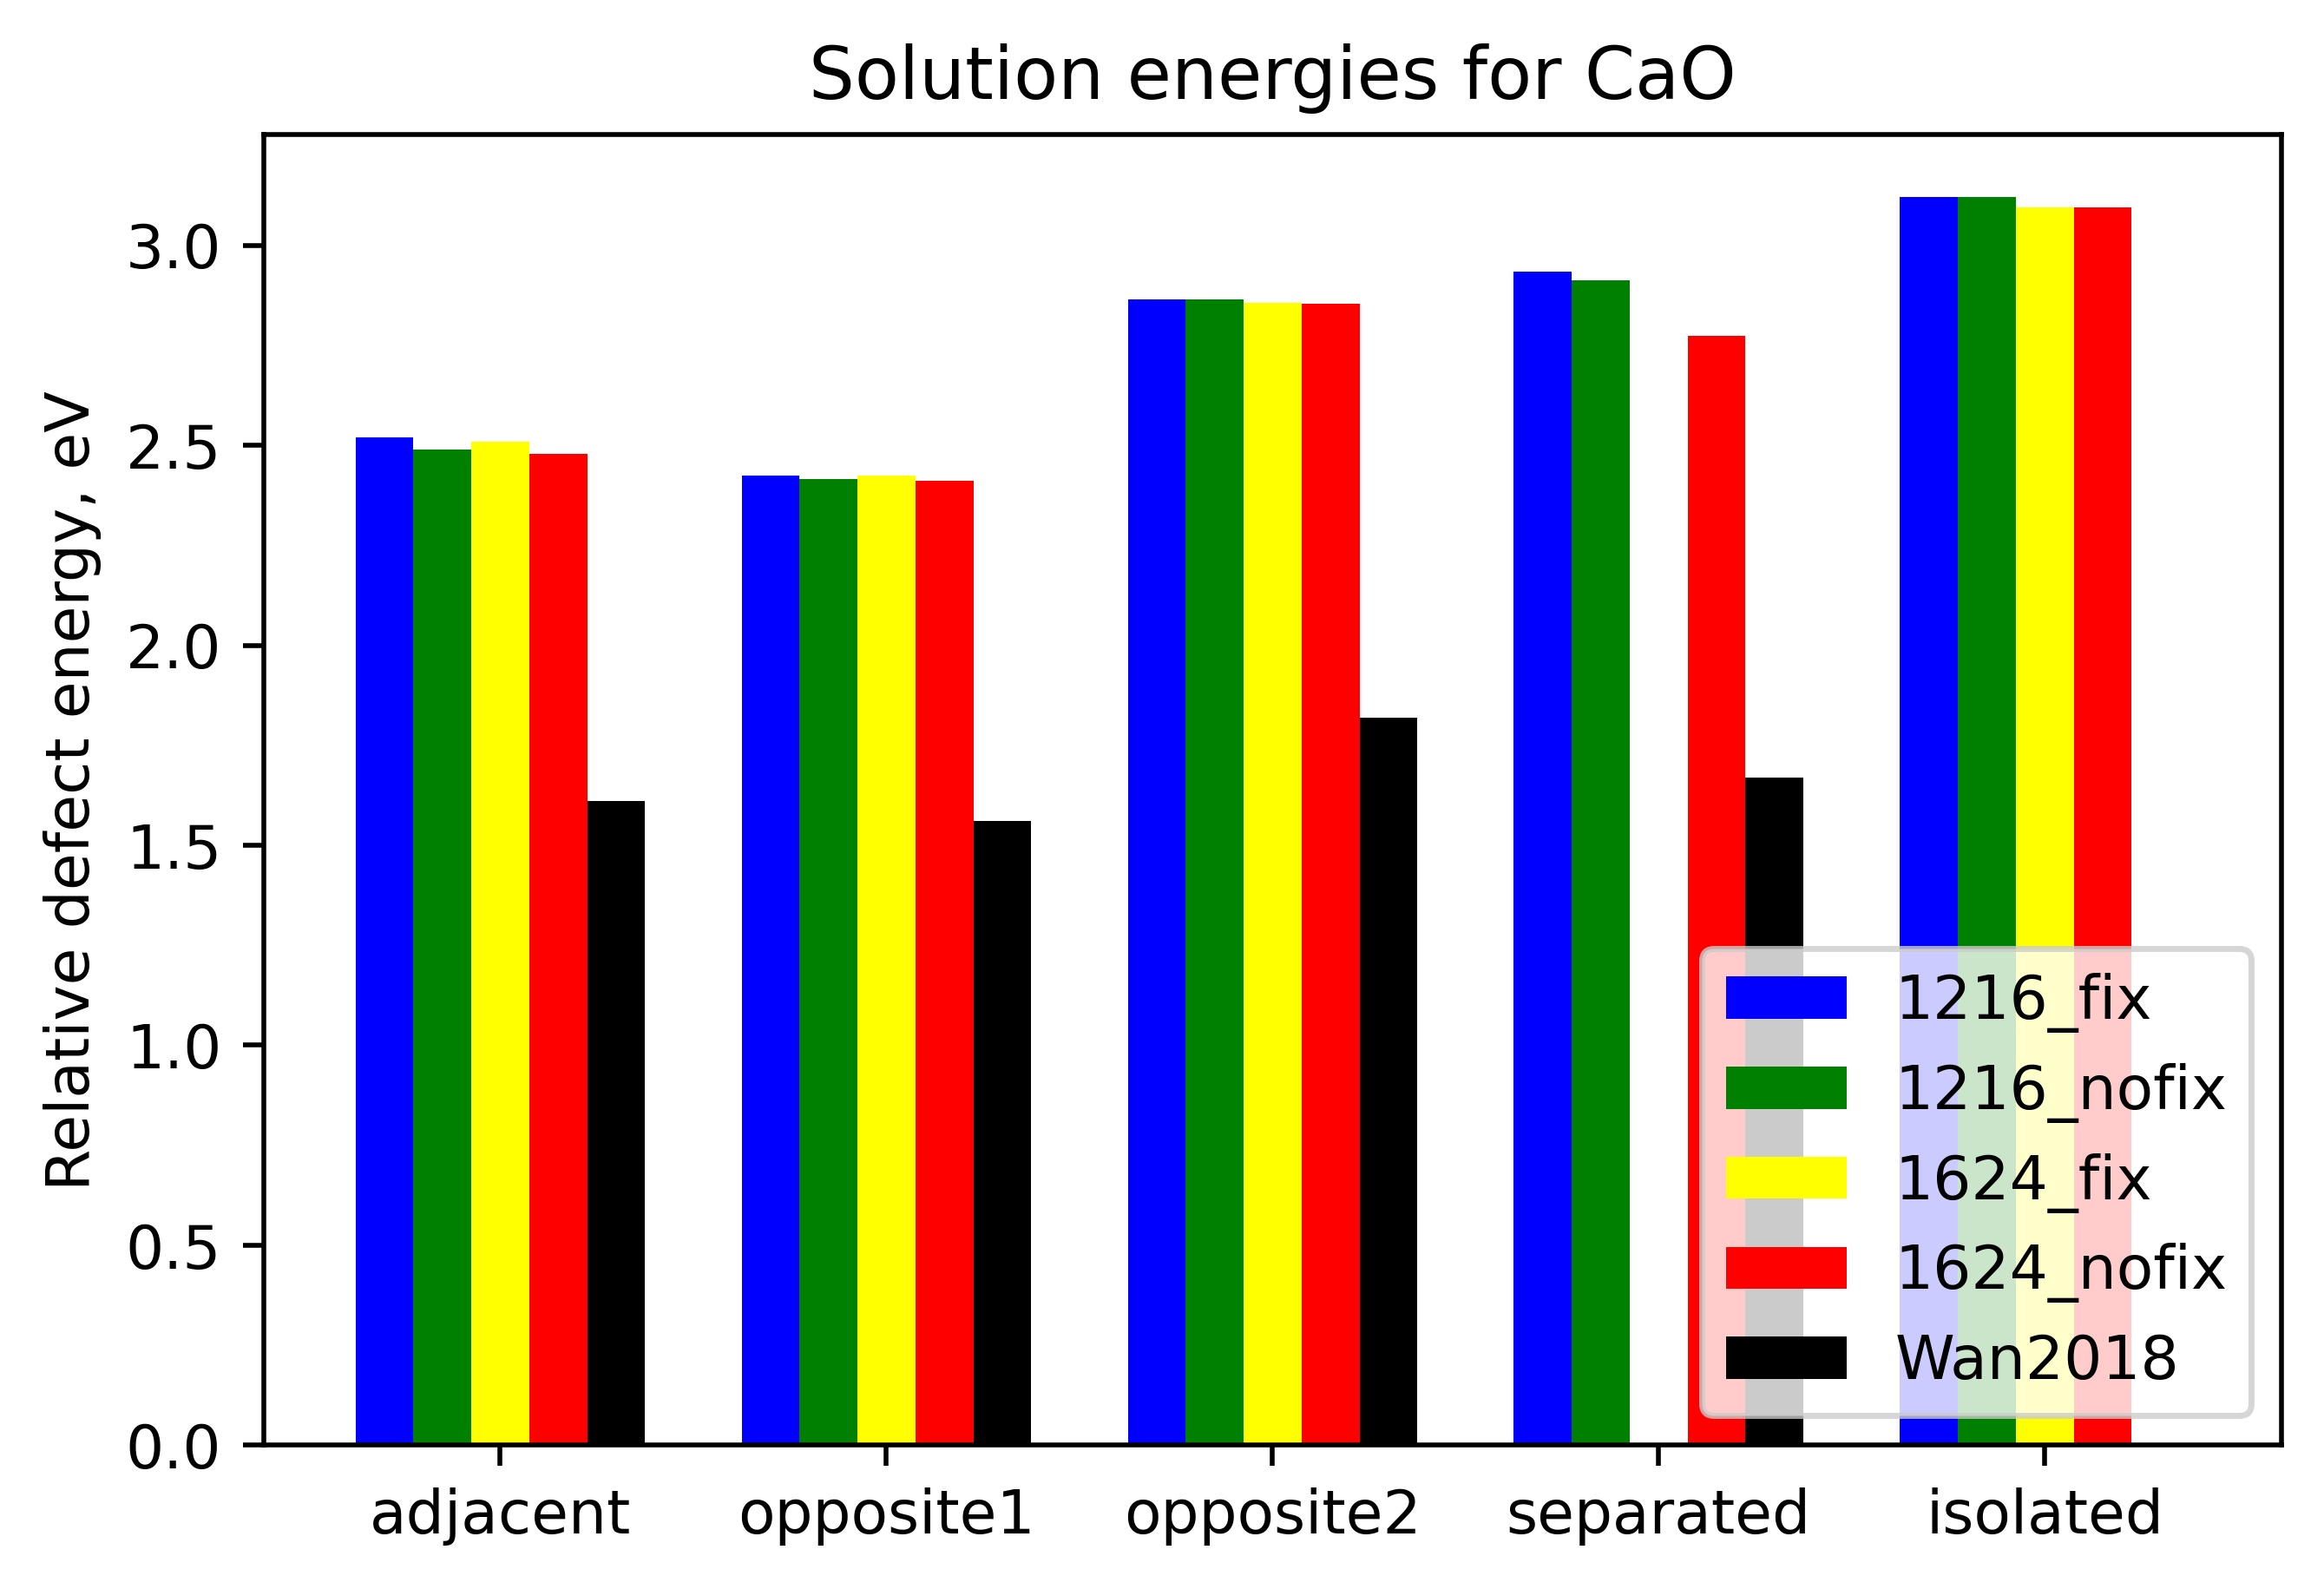
\includegraphics[width=0.4\textwidth]{ca_absolute.jpg}
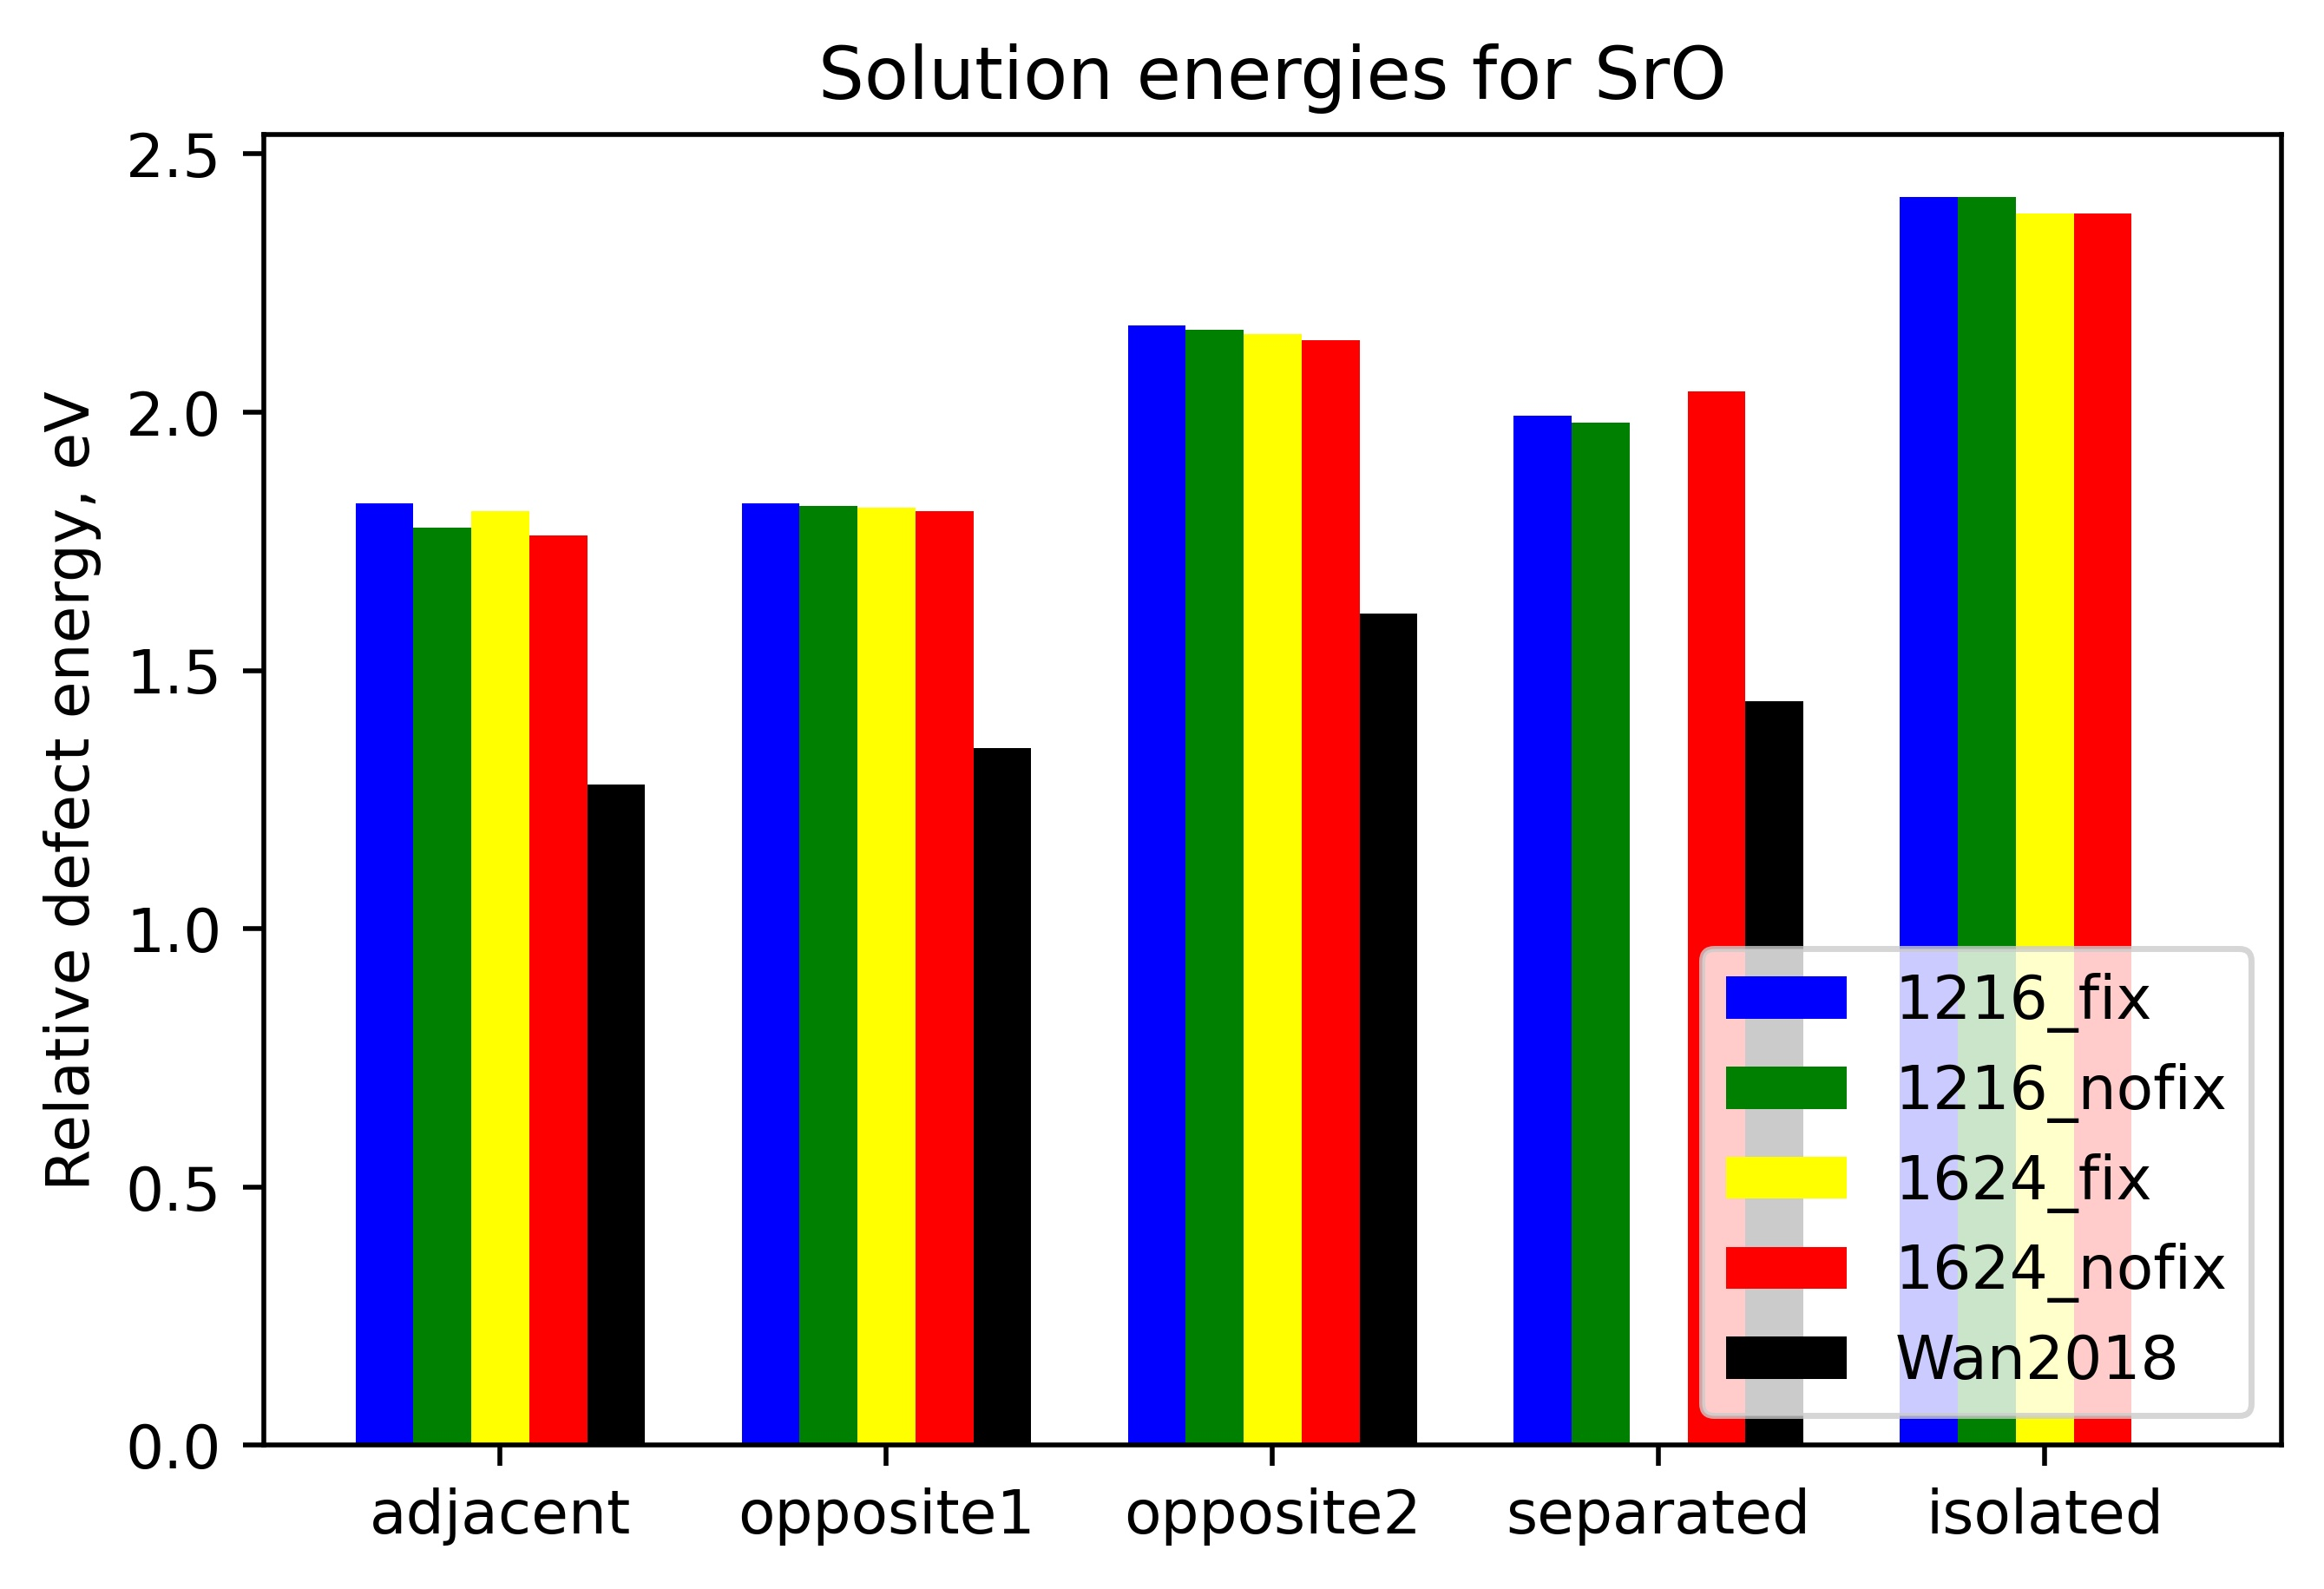
\includegraphics[width=0.4\textwidth]{sr_absolute.jpg}
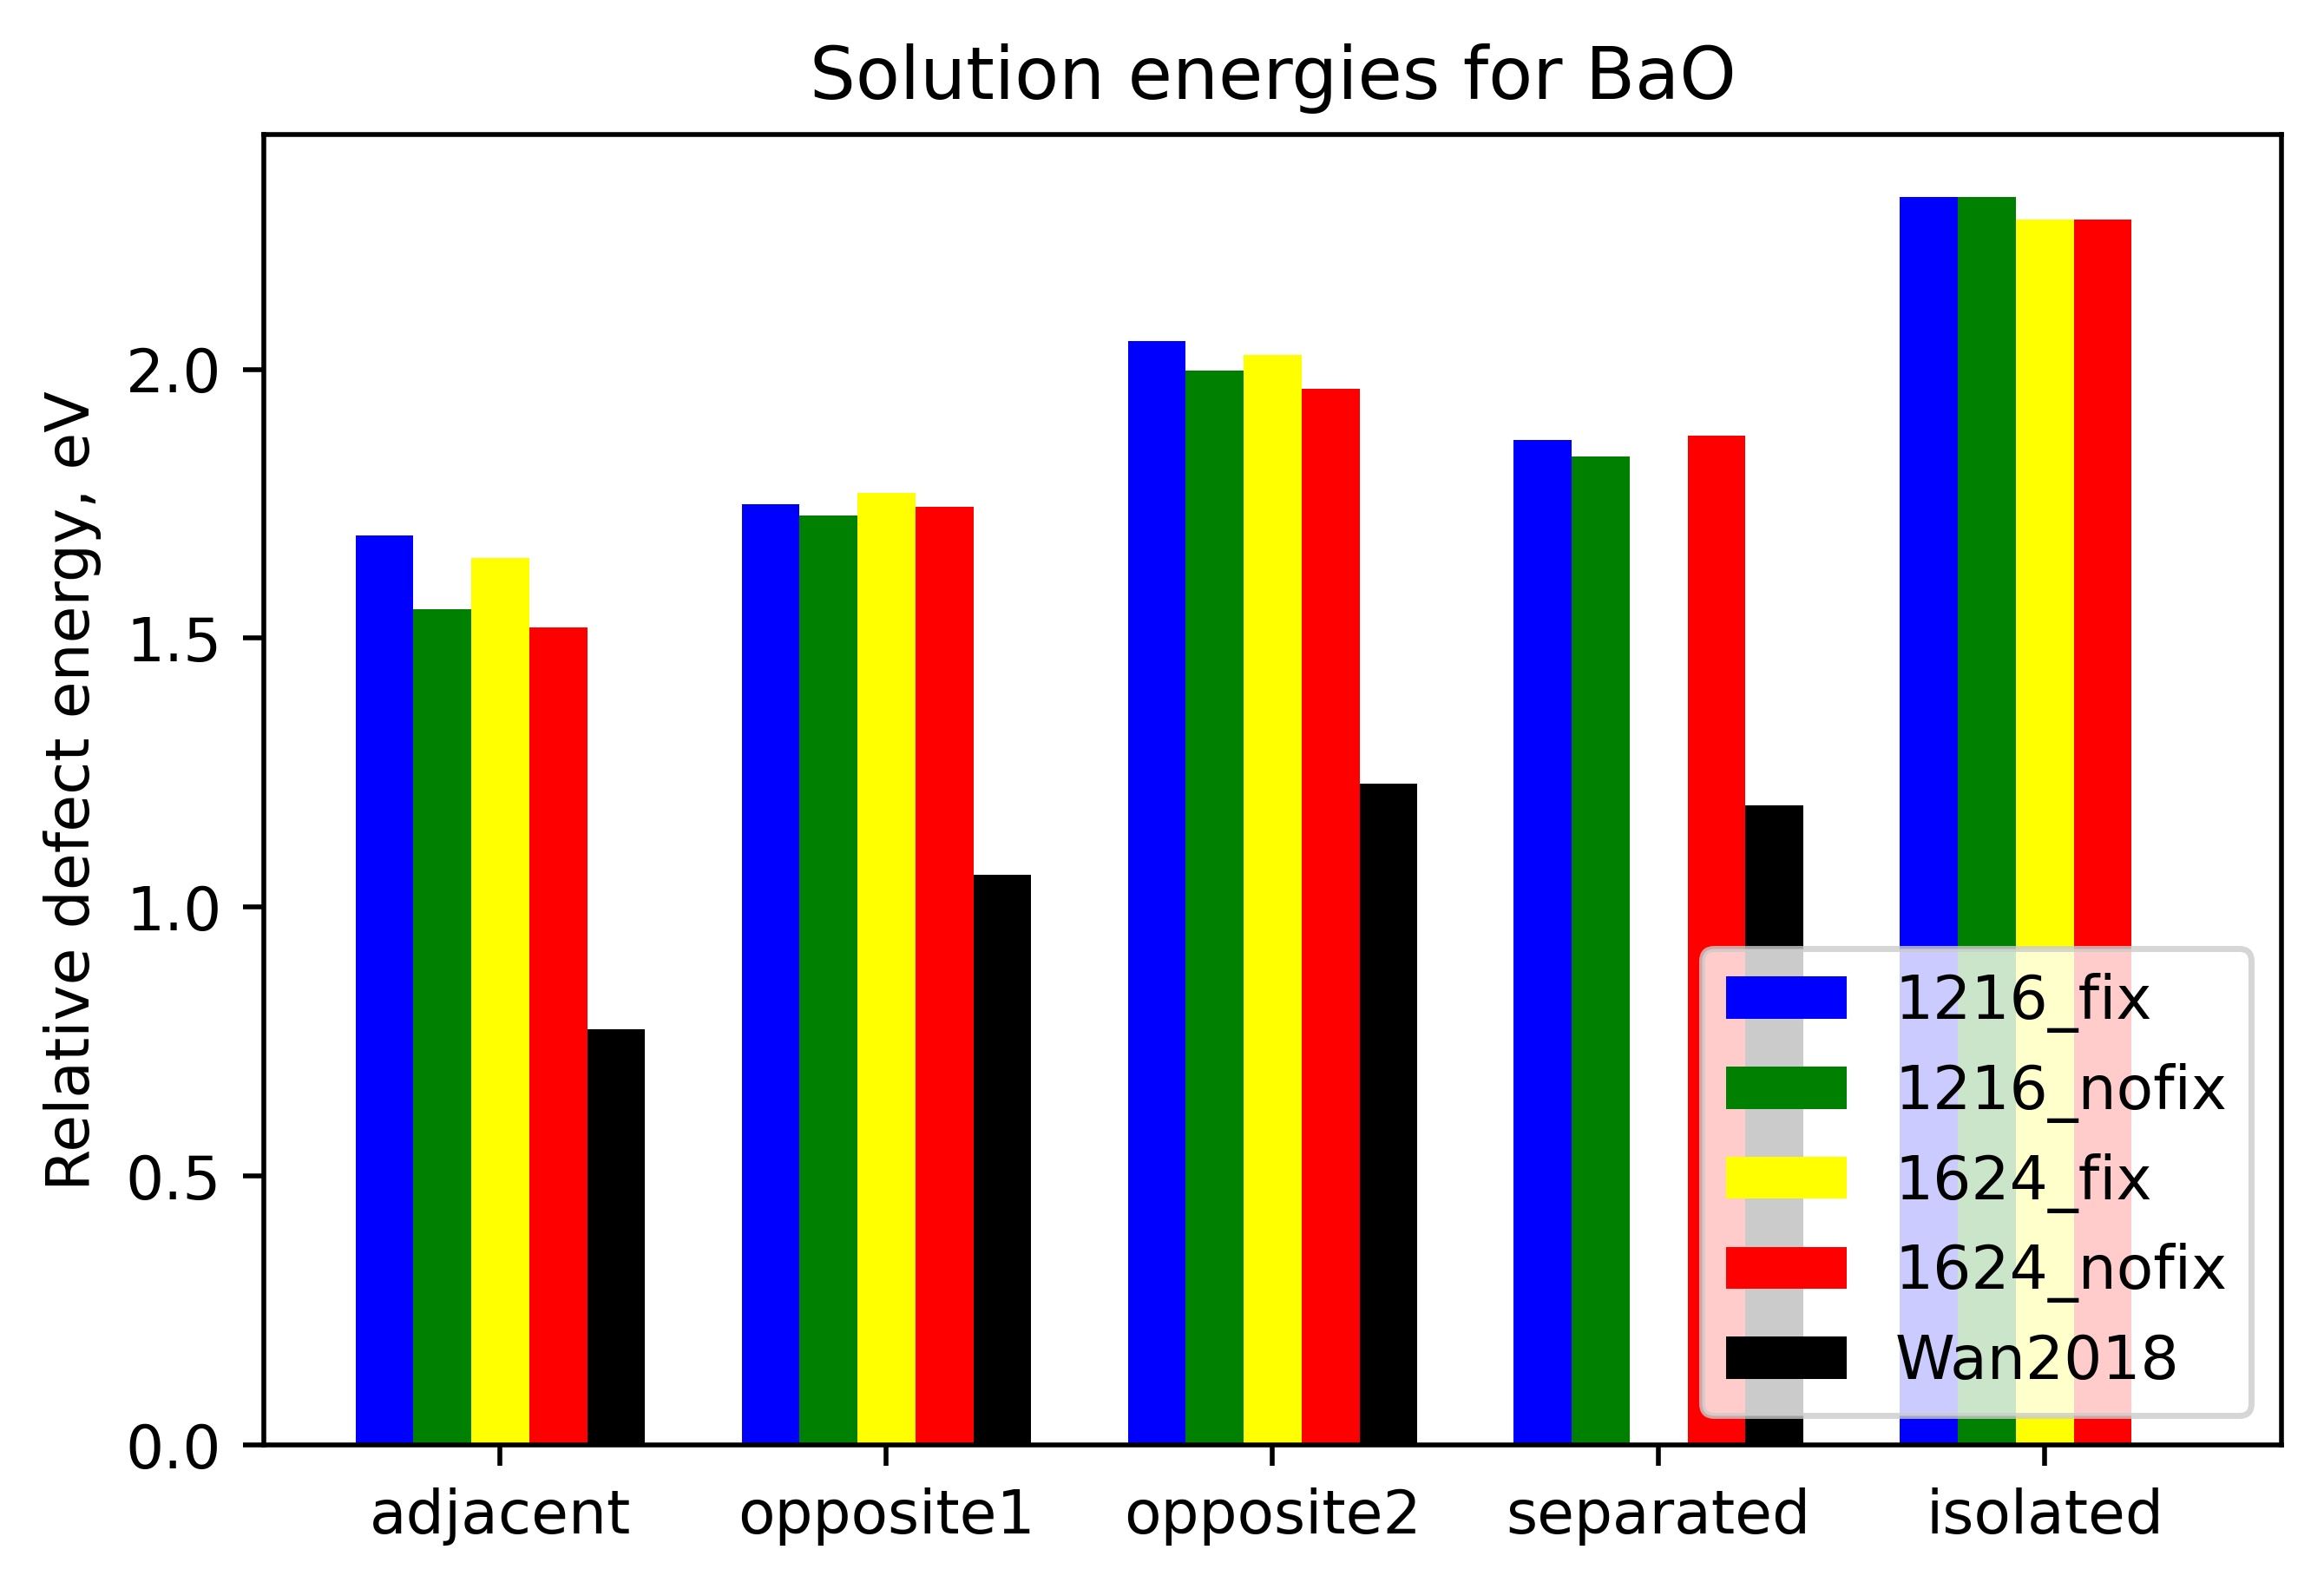
\includegraphics[width=0.4\textwidth]{ba_absolute.jpg}
\end{figure}

\end{frame}
\begin{frame}
\frametitle{Doping Configurations}

\begin{figure}
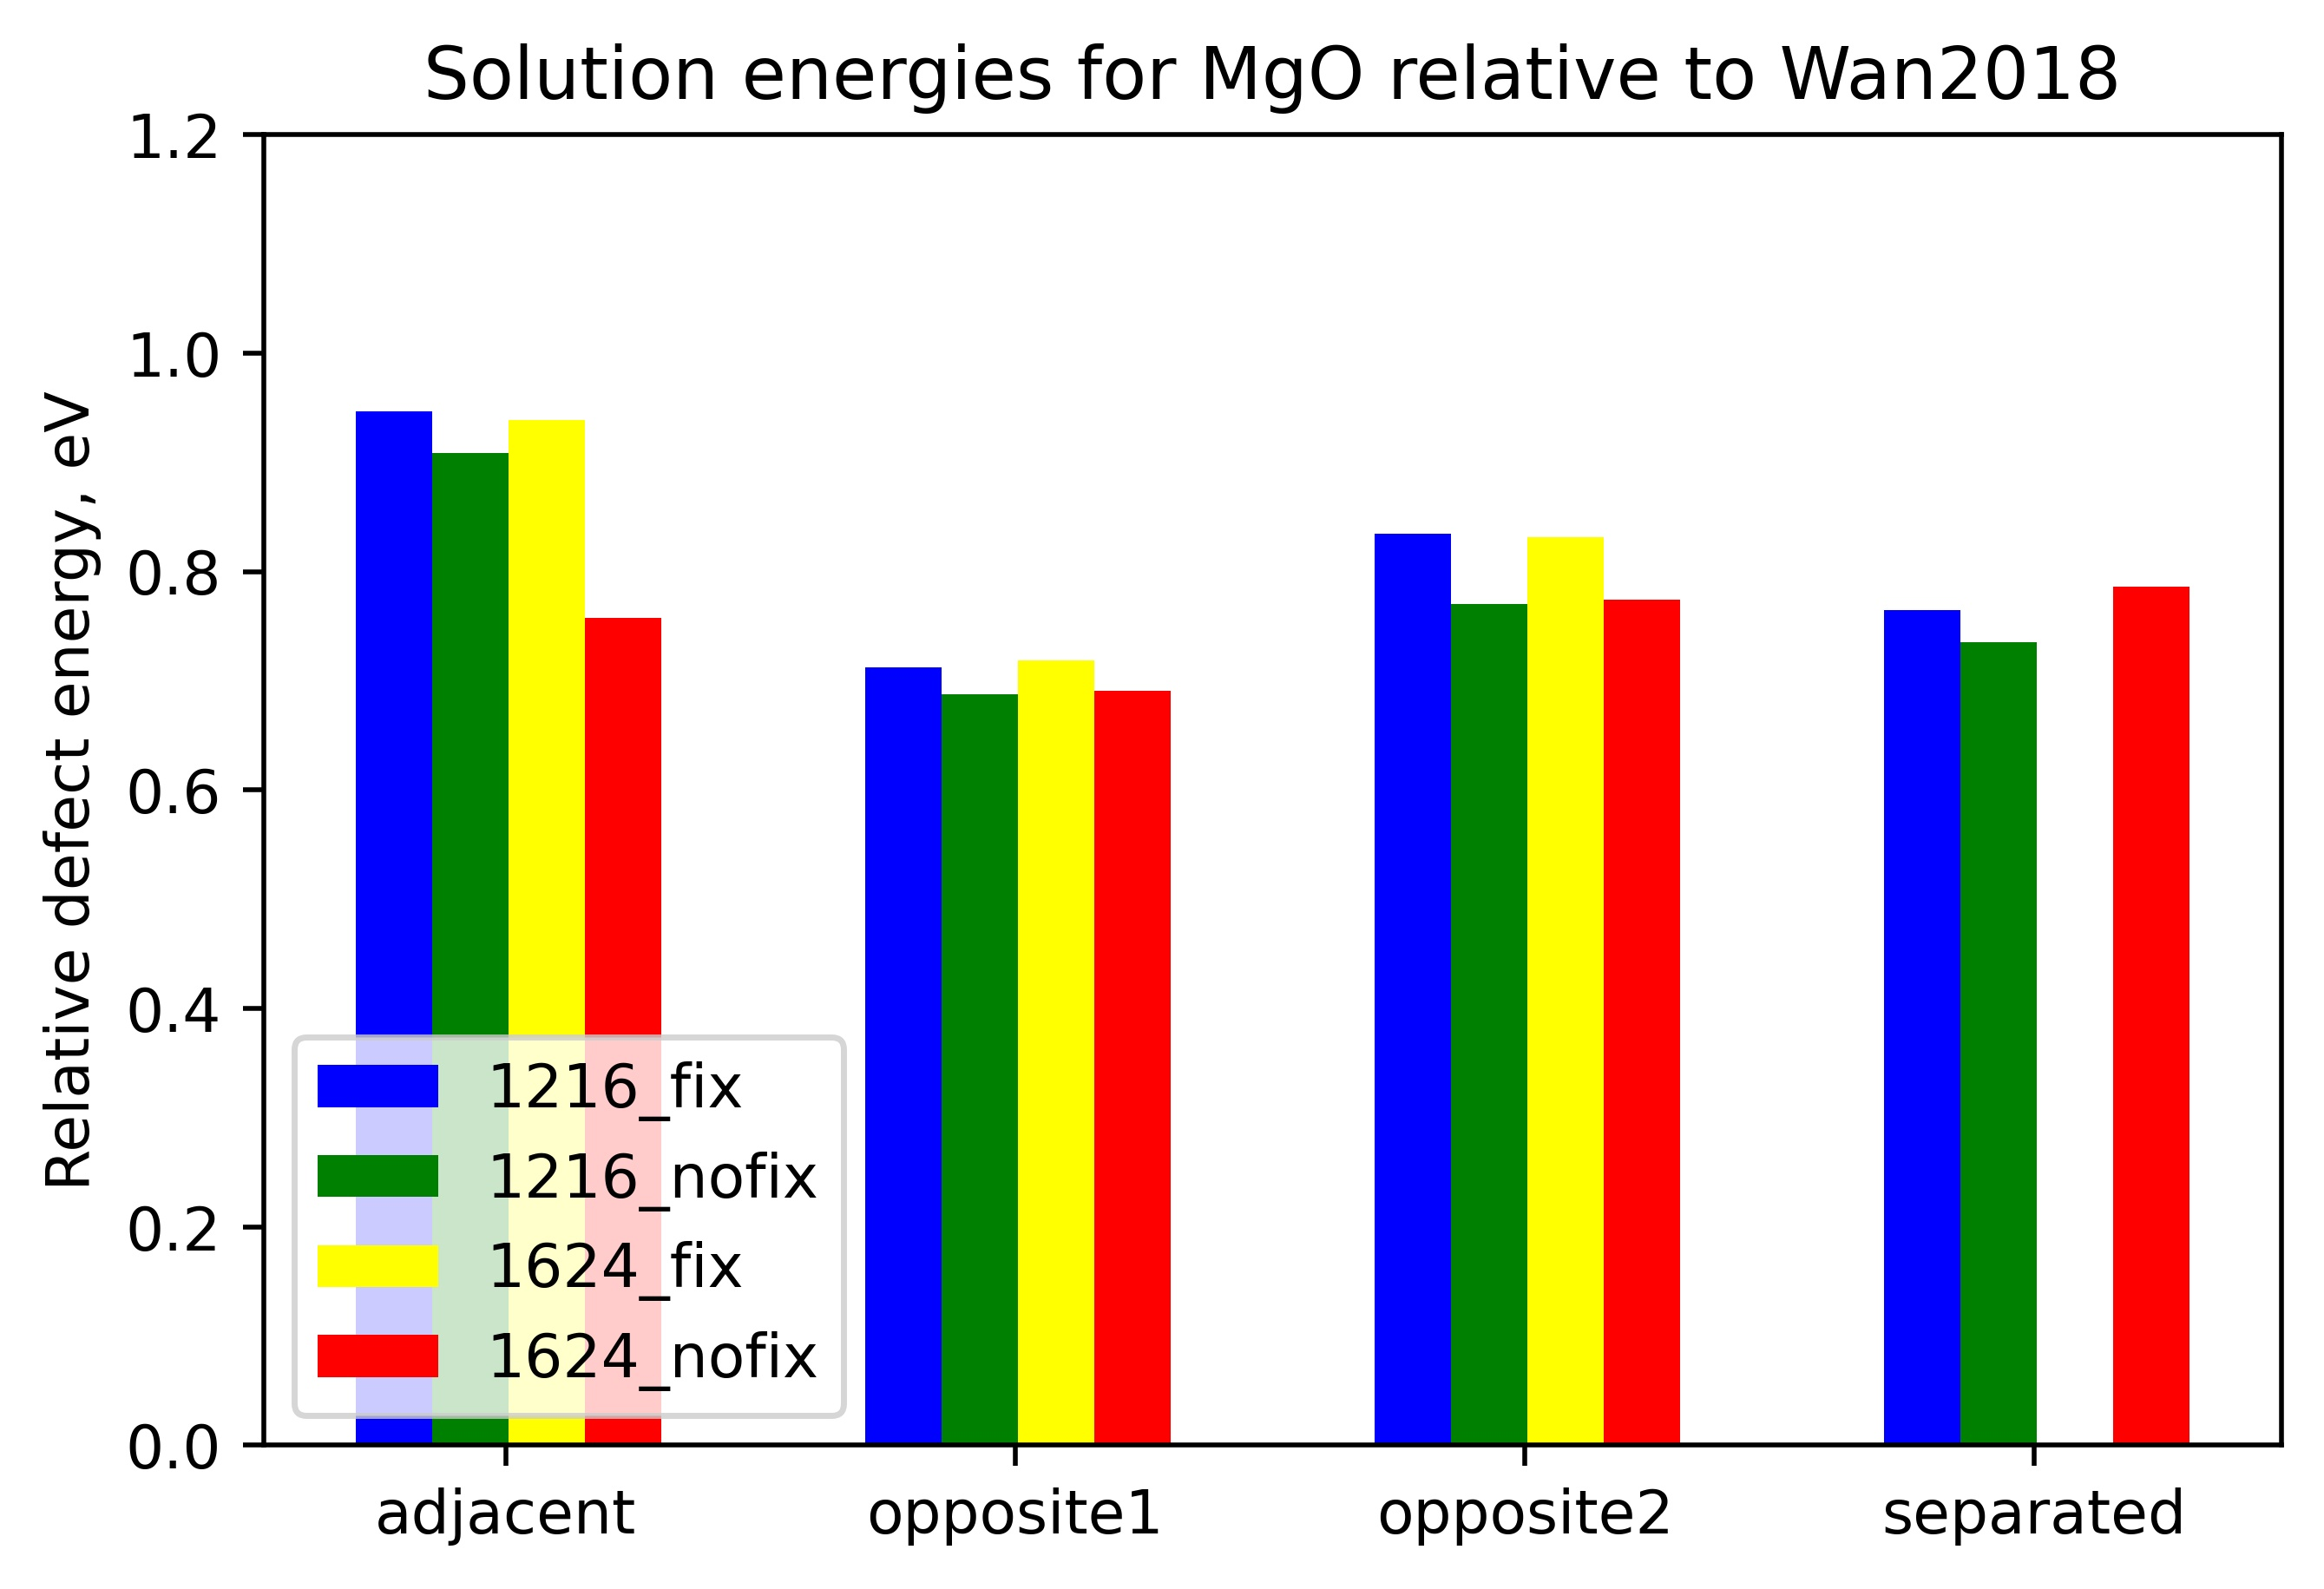
\includegraphics[width=0.4\textwidth]{mg_relative.jpg}
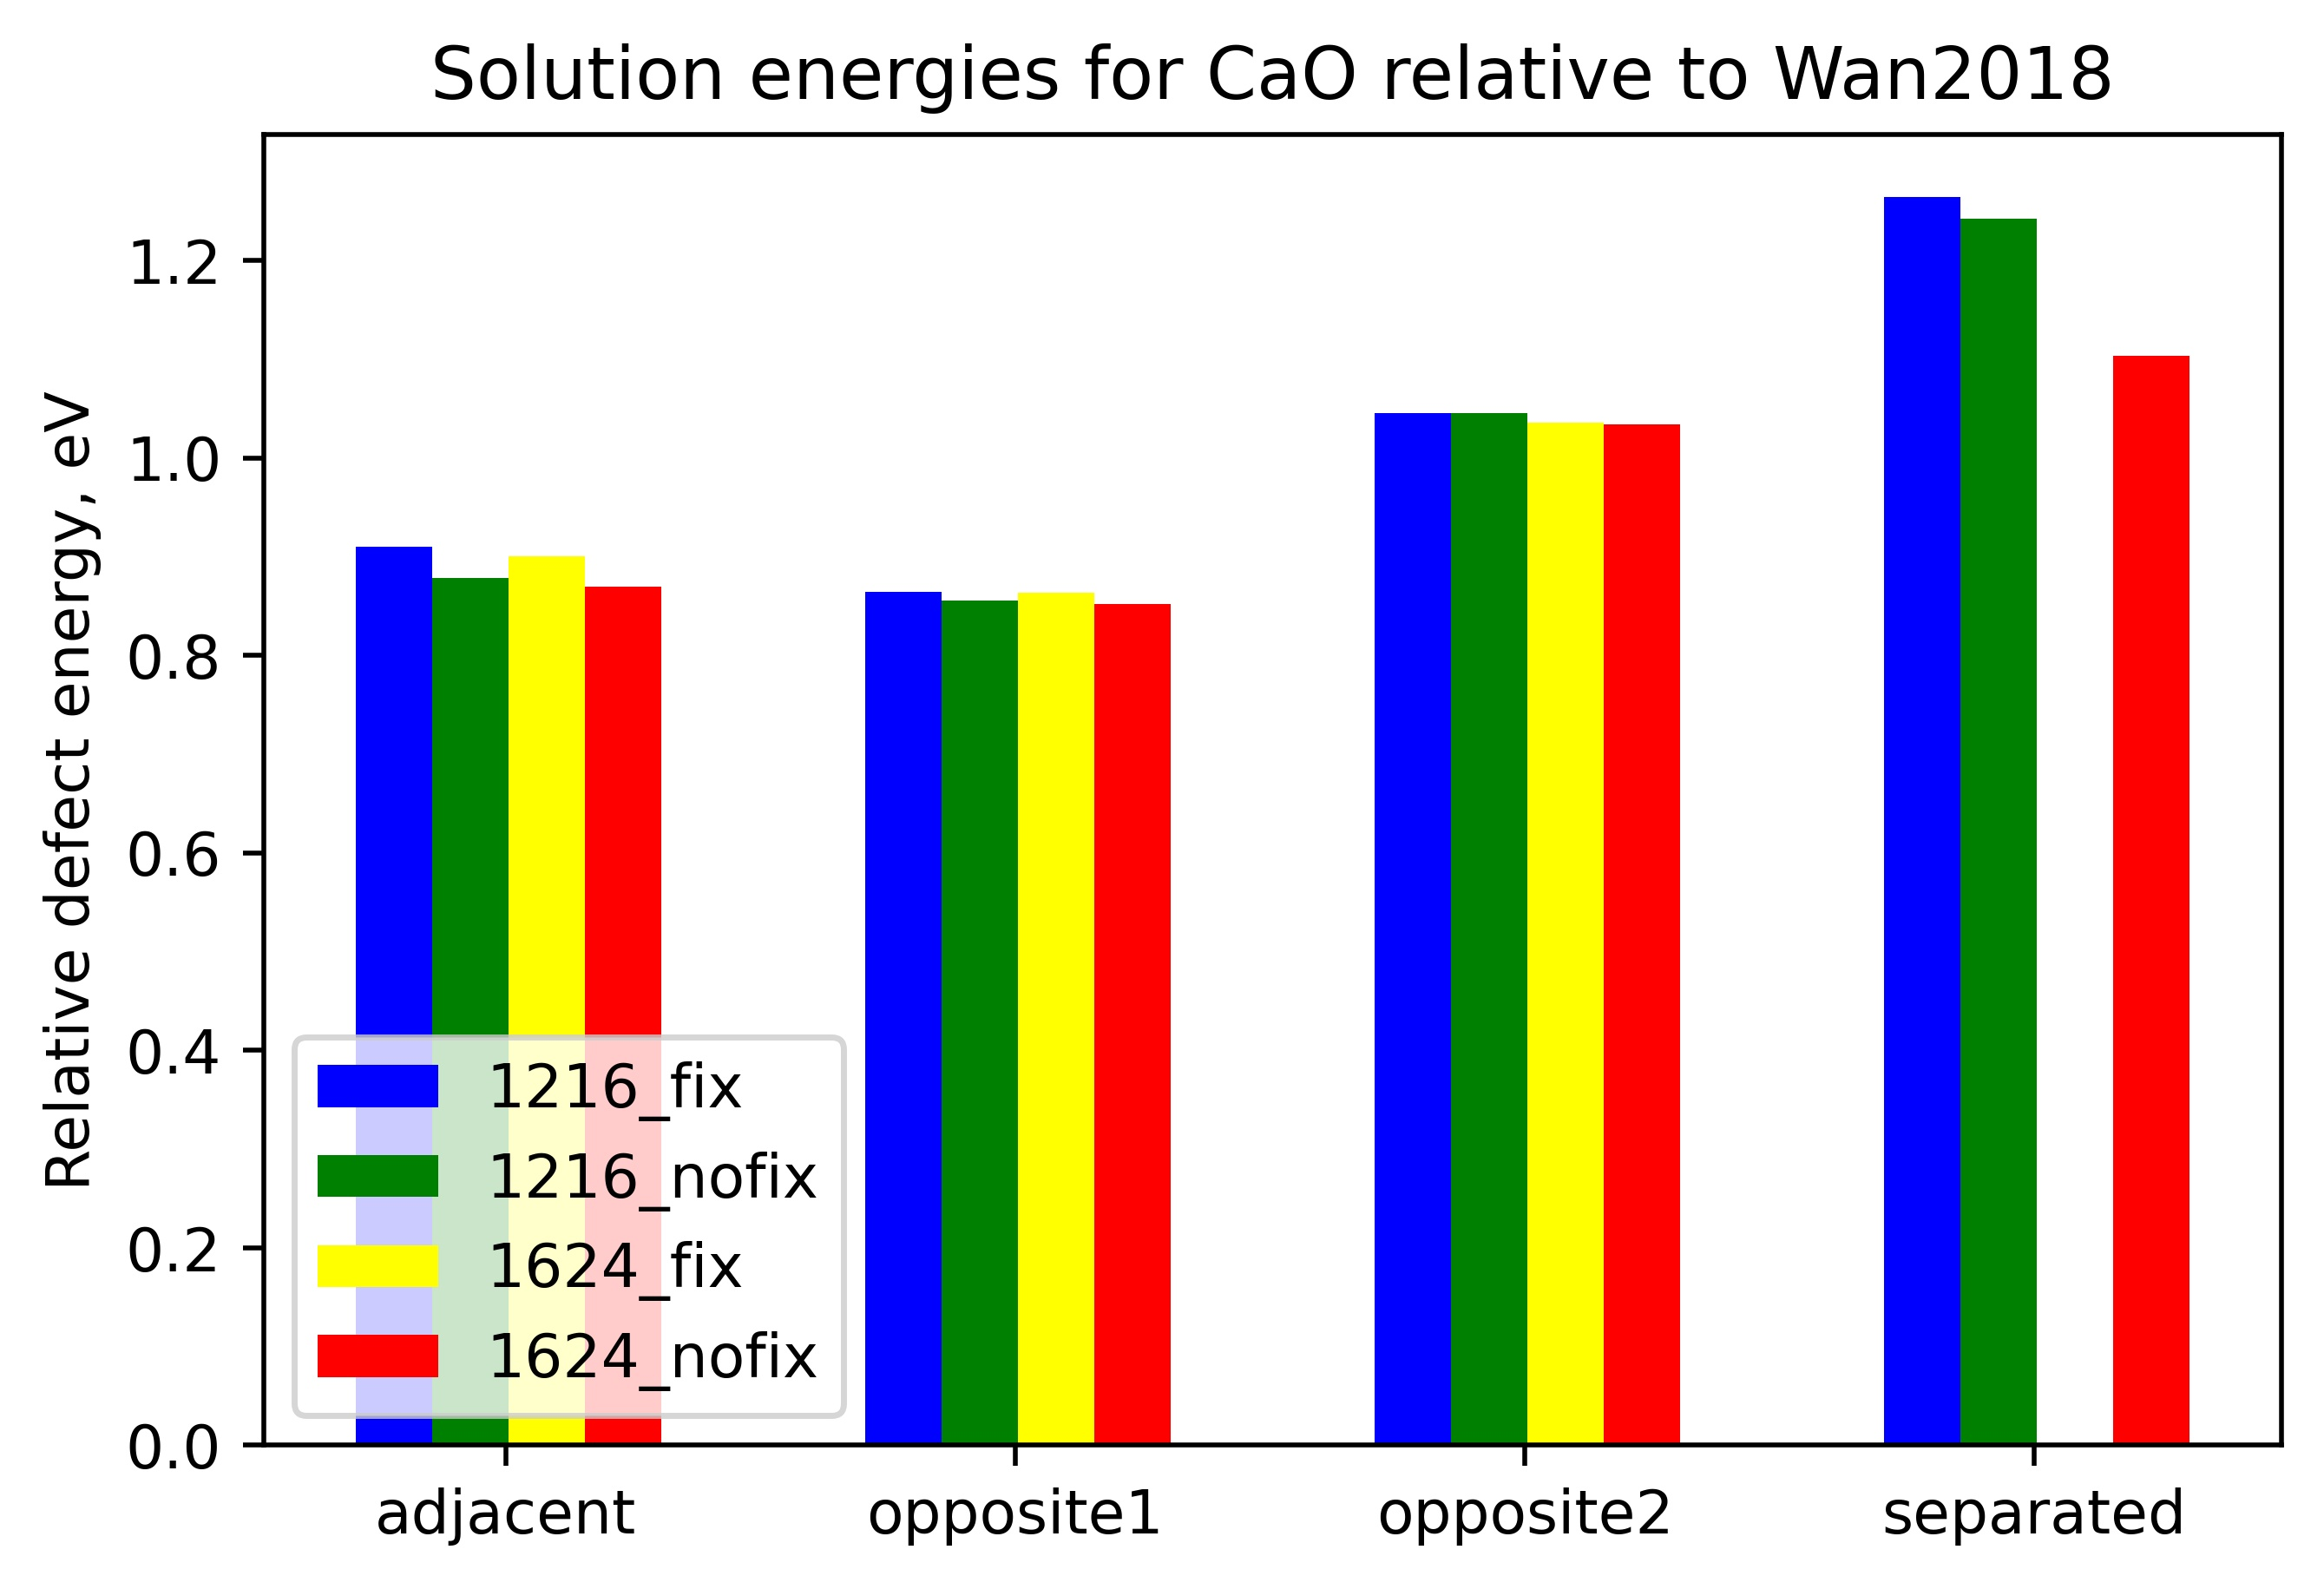
\includegraphics[width=0.4\textwidth]{ca_relative.jpg}
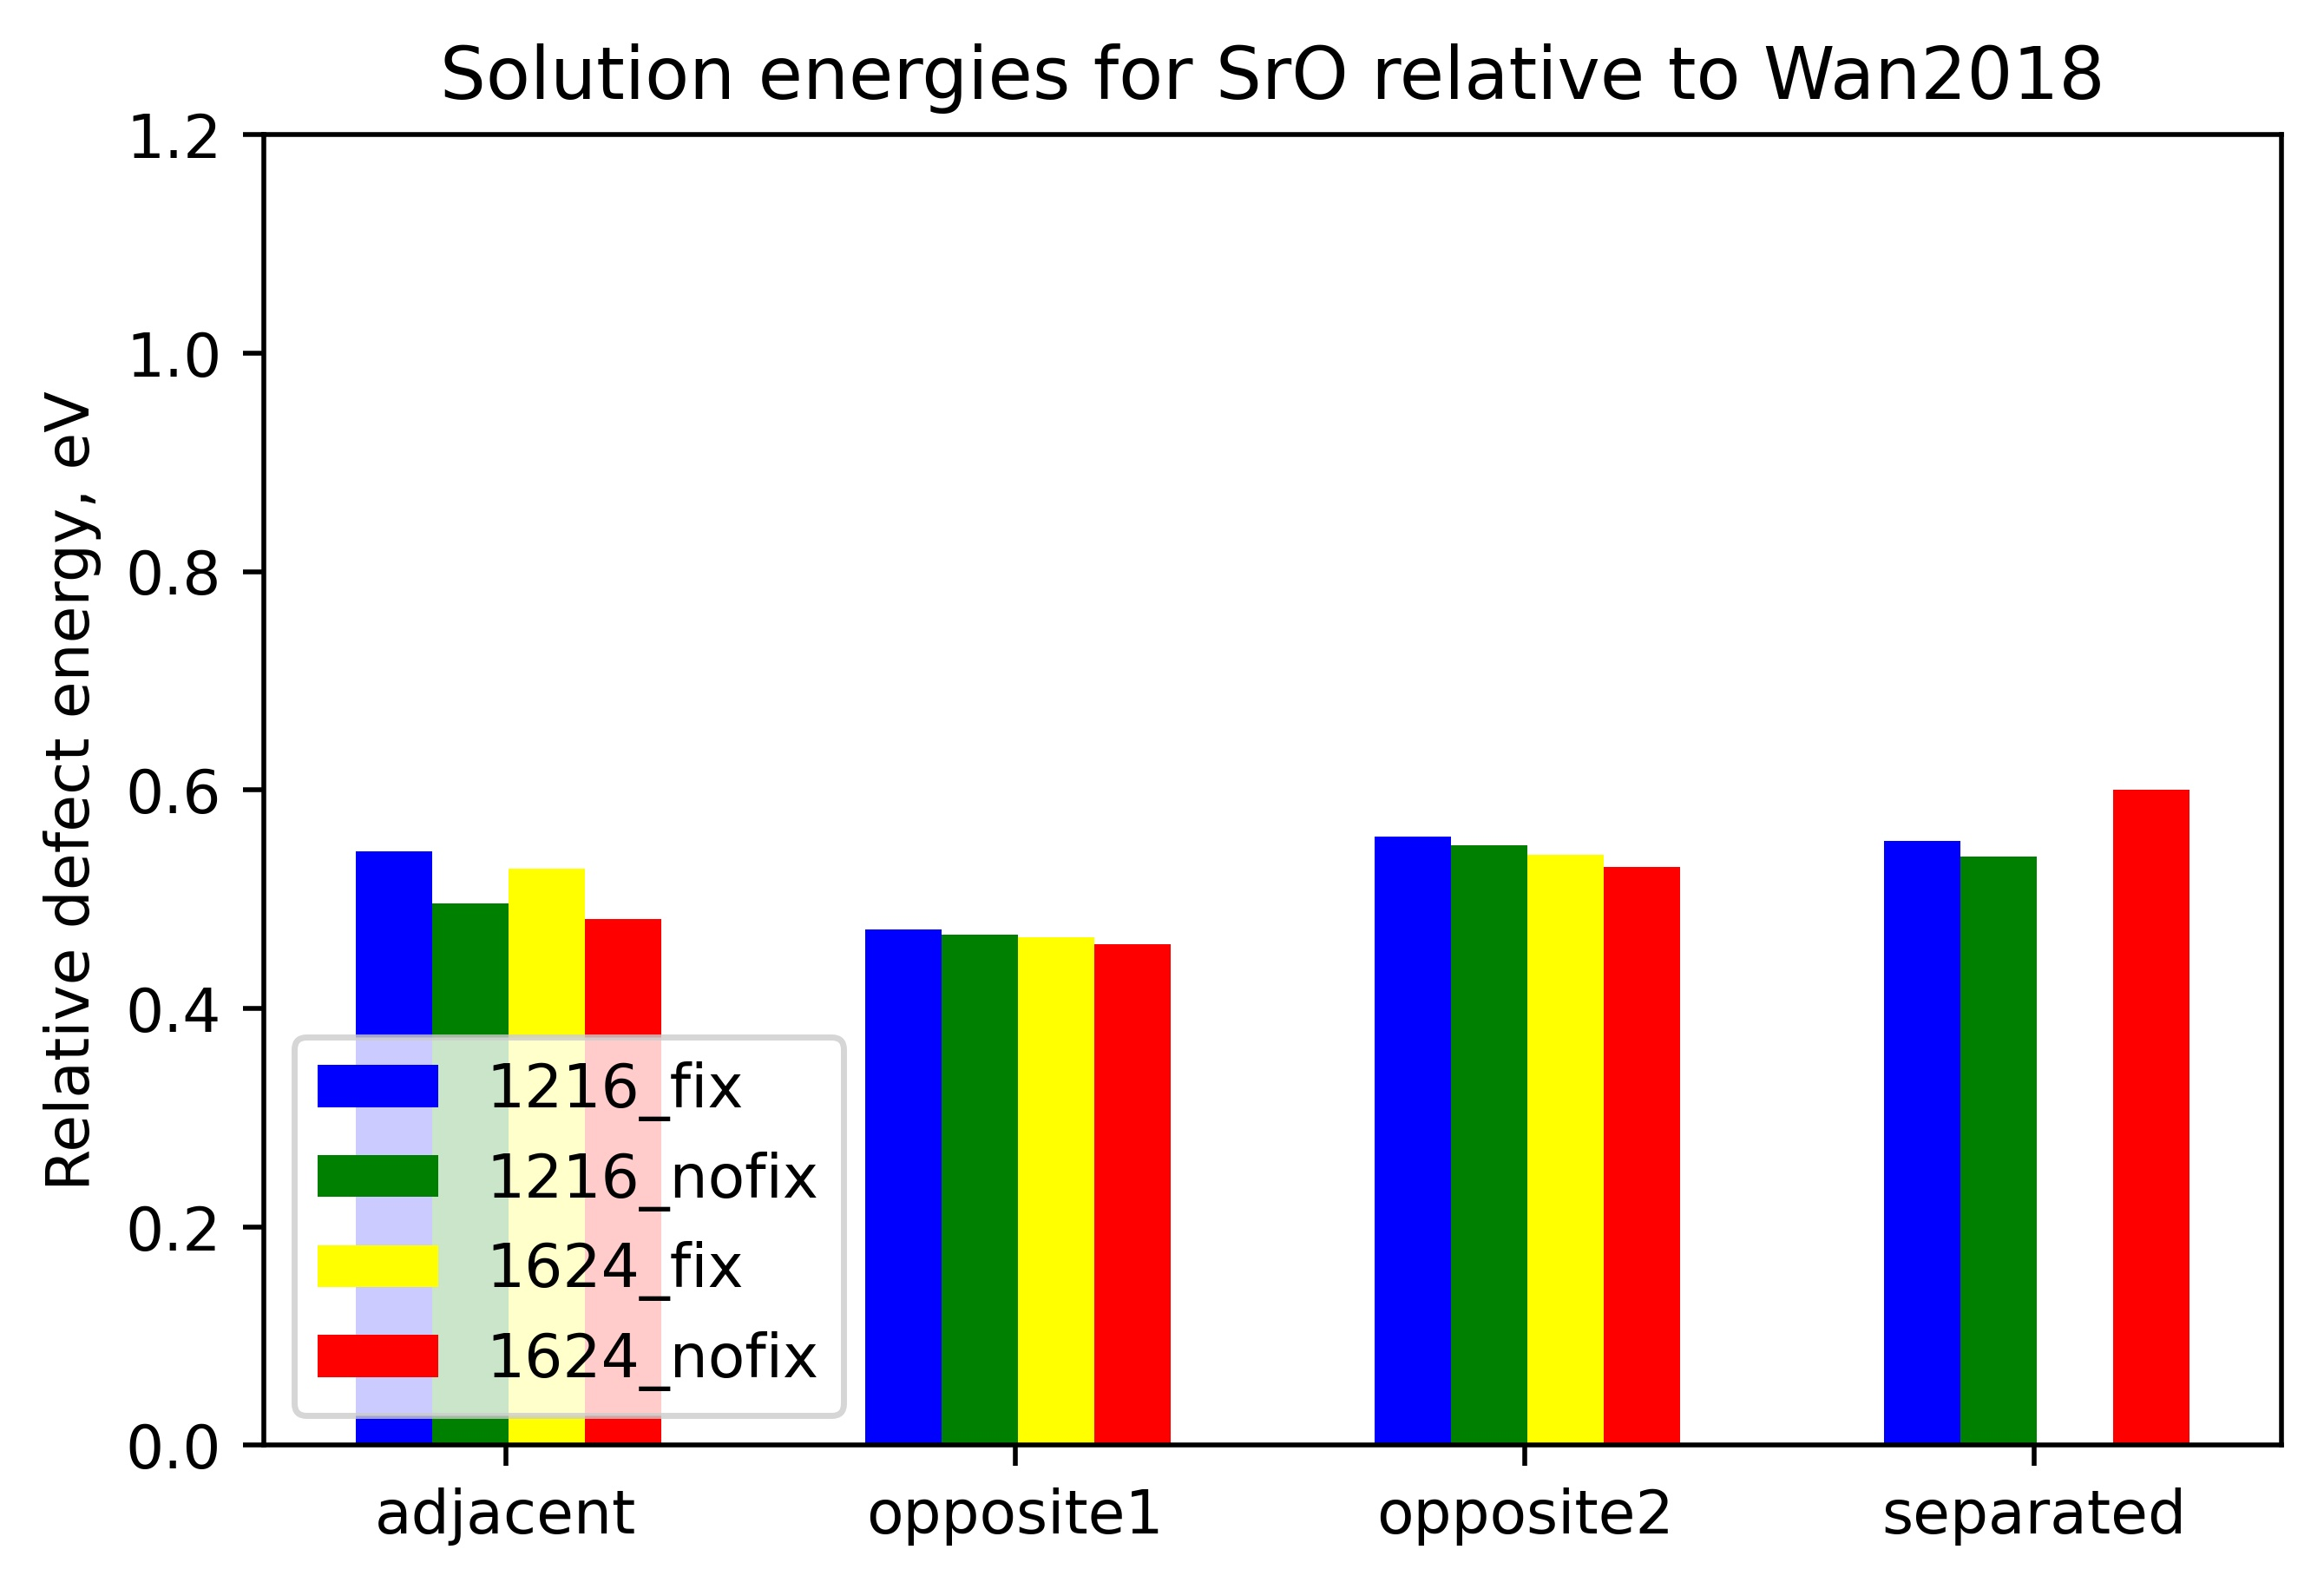
\includegraphics[width=0.4\textwidth]{sr_relative.jpg}
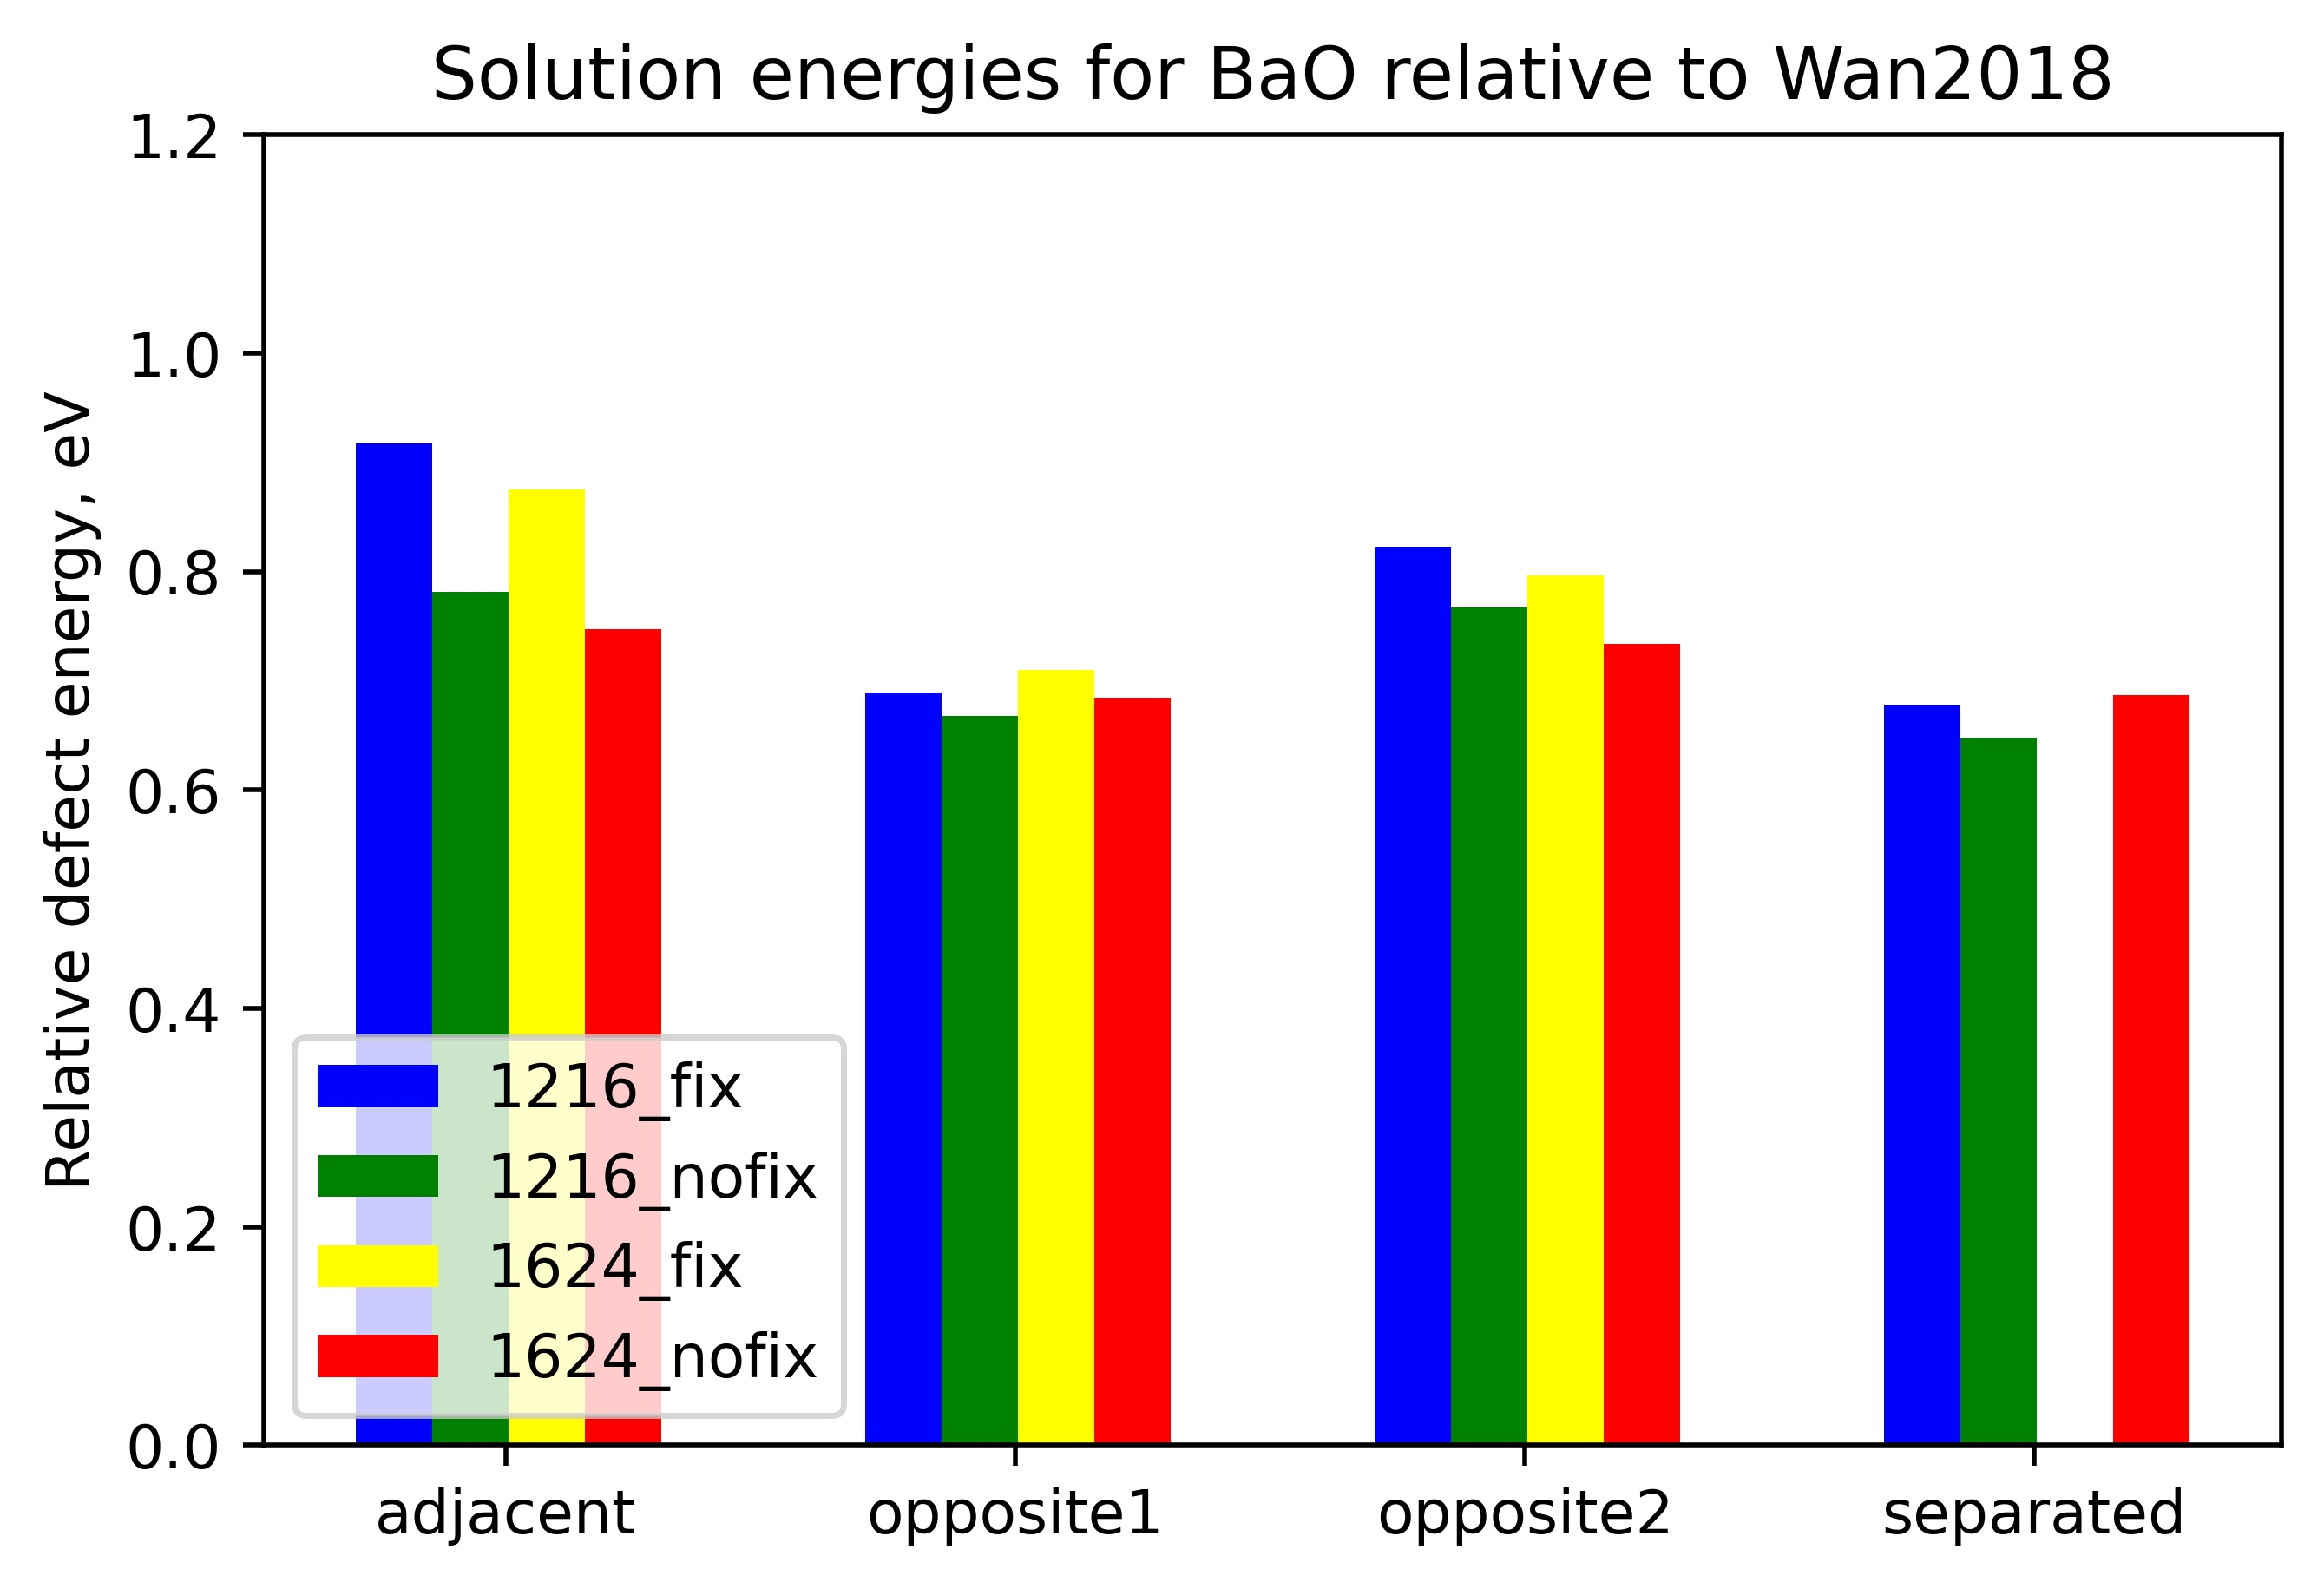
\includegraphics[width=0.4\textwidth]{ba_relative.jpg}
\end{figure}

\end{frame}

\begin{frame}
\frametitle{Clustering}

\begin{figure}
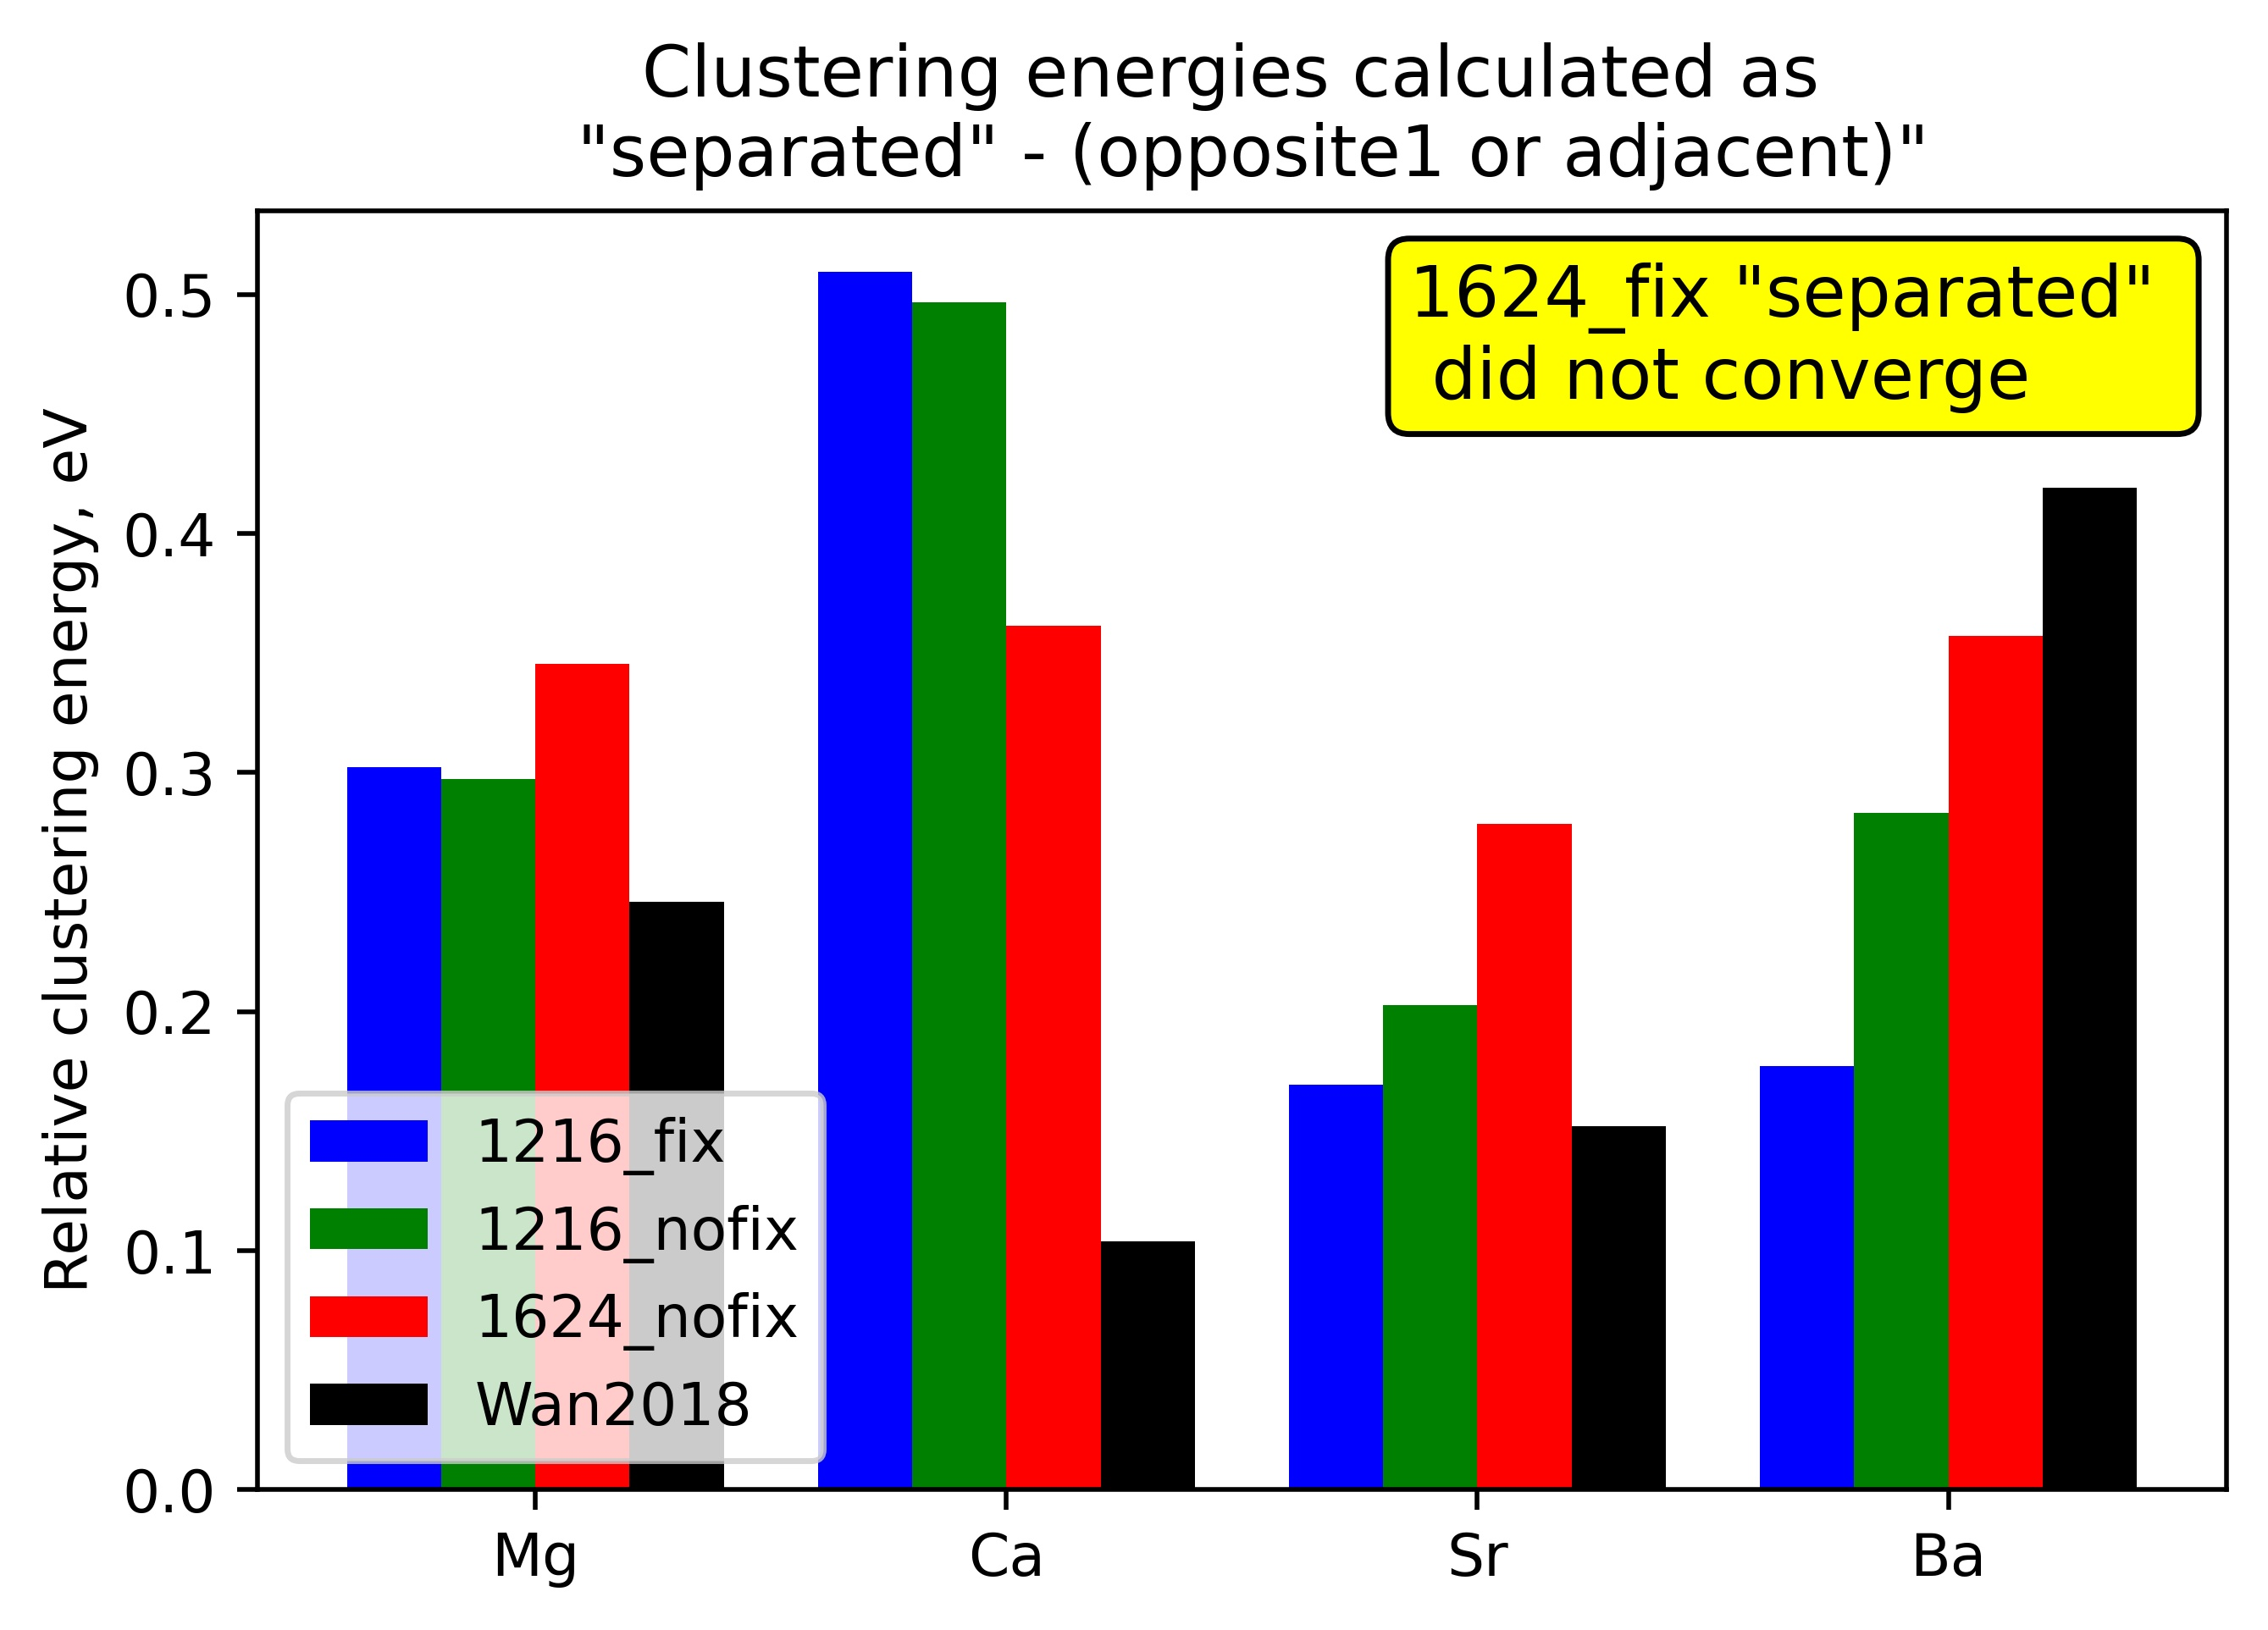
\includegraphics[width=0.4\textwidth]{clustering.jpg}
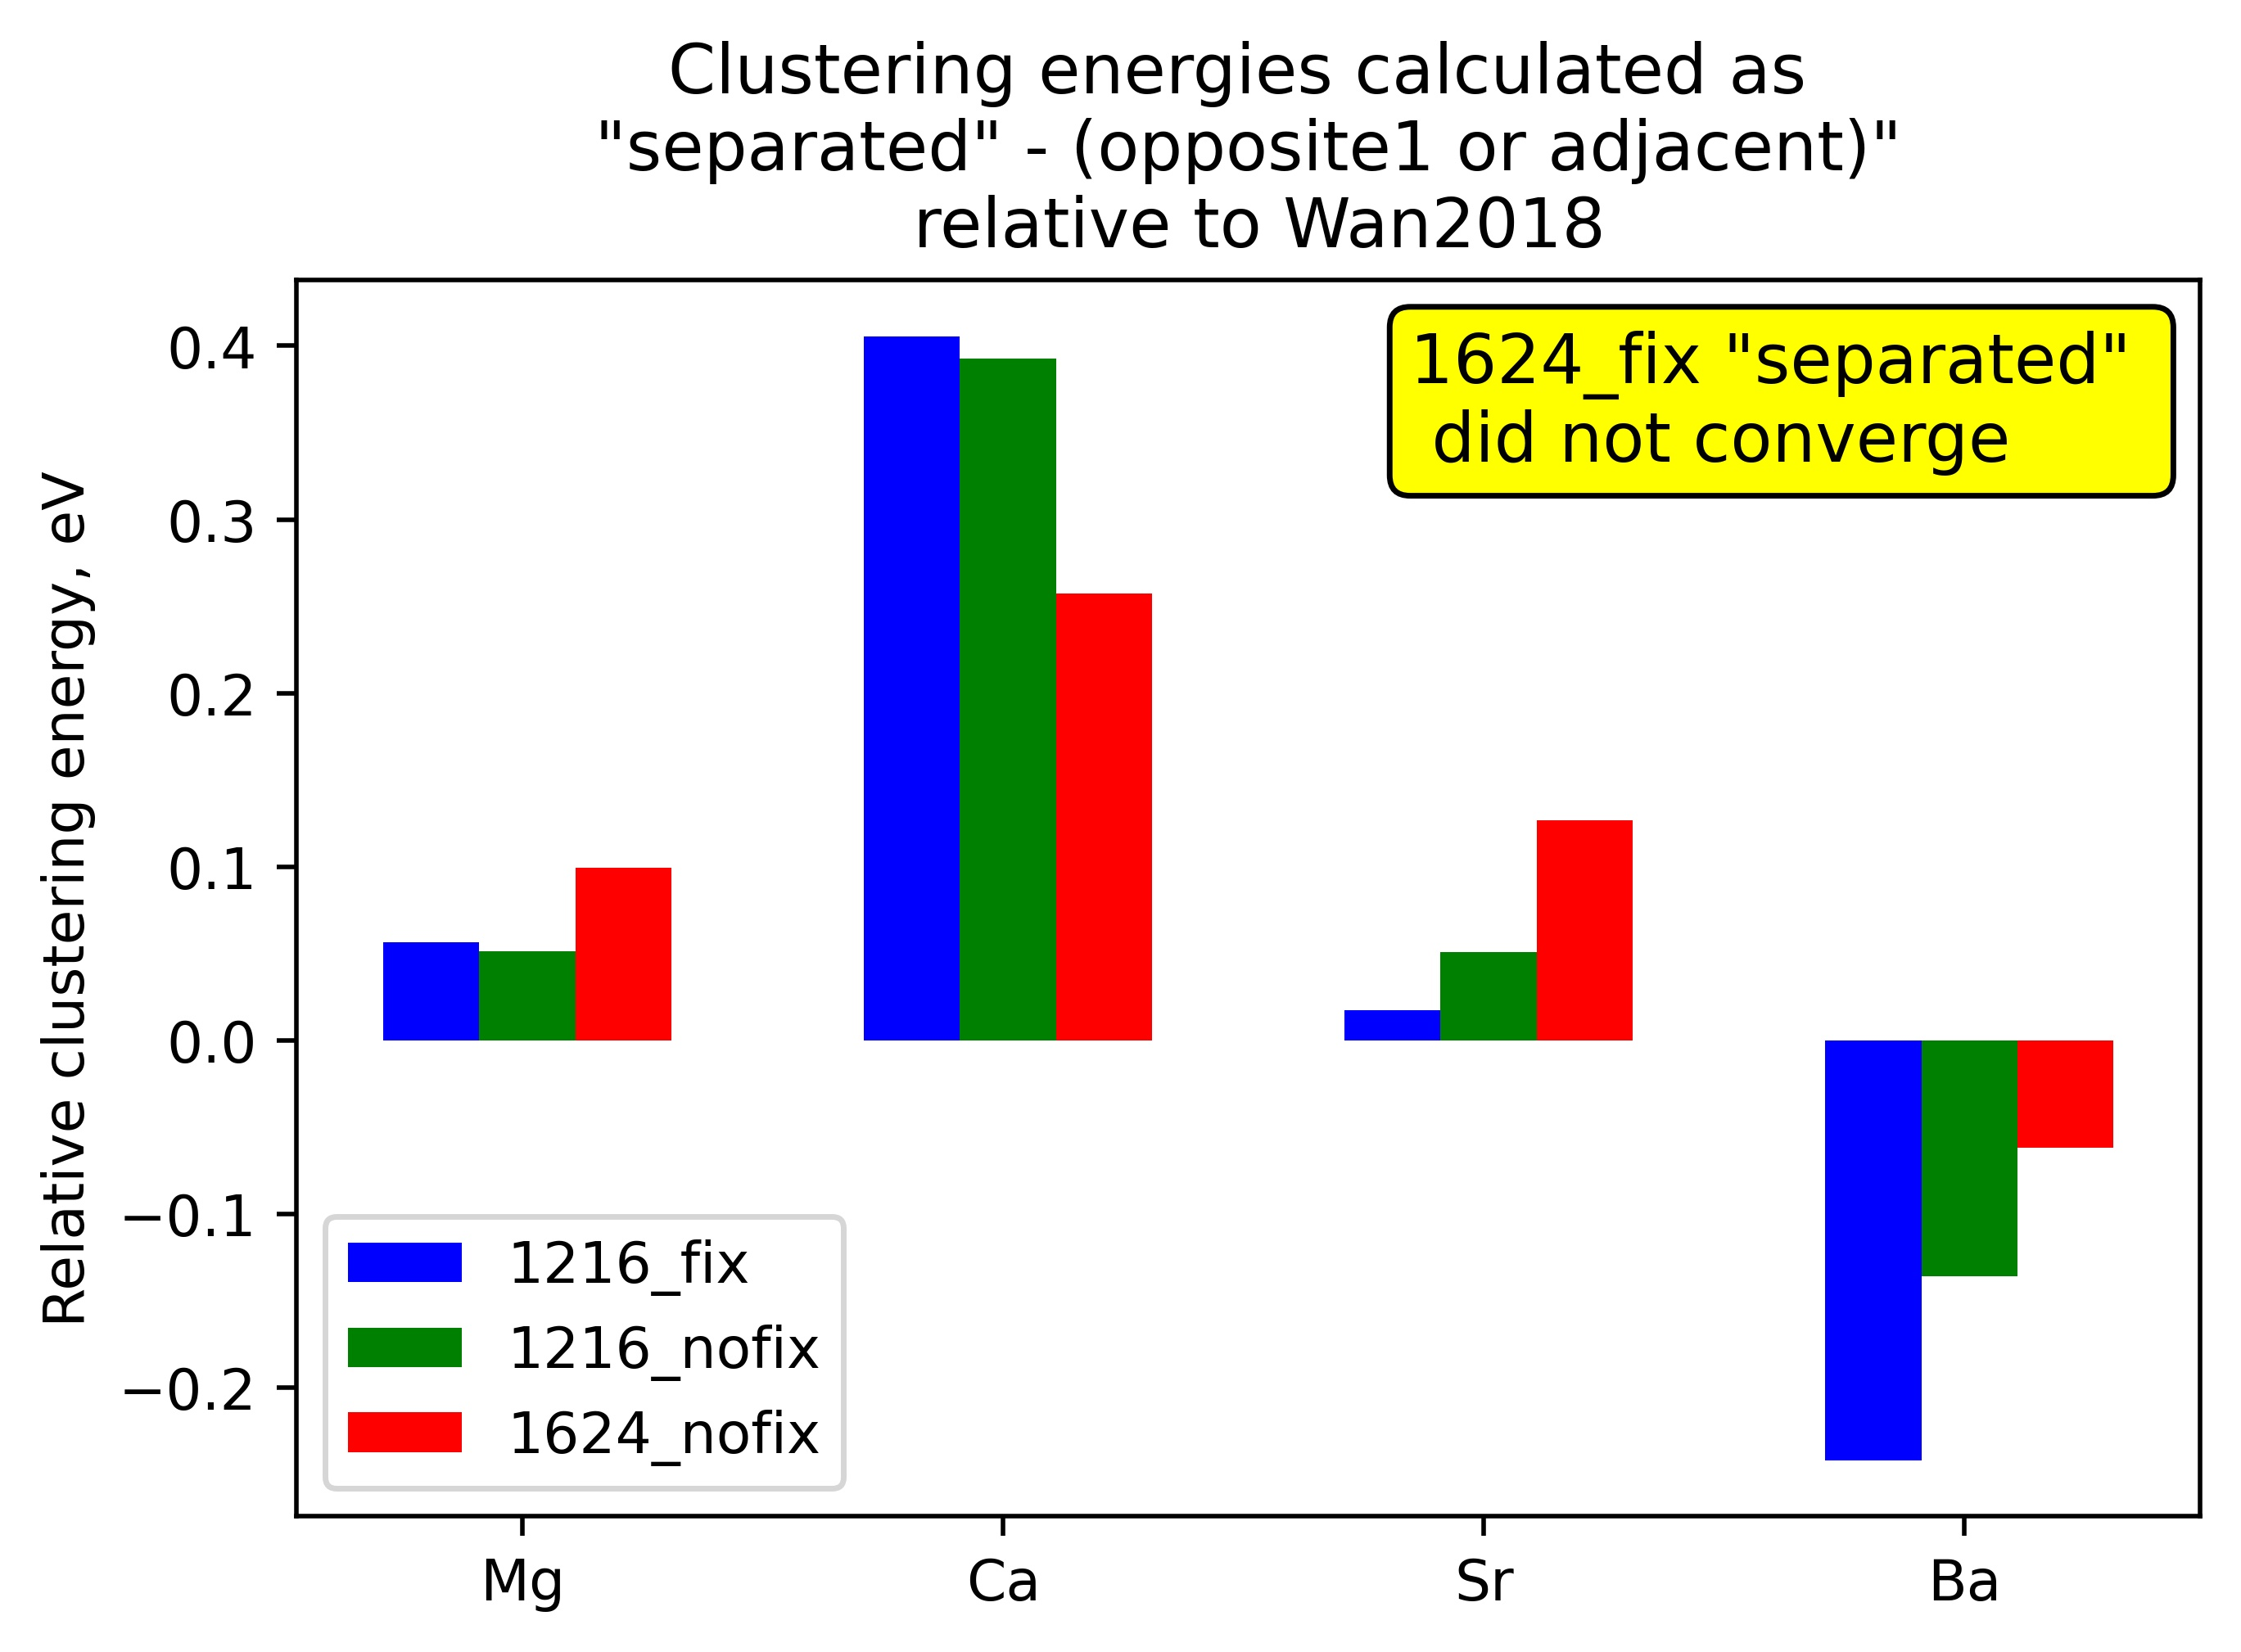
\includegraphics[width=0.4\textwidth]{clustering_relative.jpg}
\end{figure}

\end{frame}

\begin{frame}
\frametitle{Next steps}

\begin{itemize}
  \item Lucy's potentials
  \item Calculations with Lucy's potentials
  \item Try MD
\end{itemize}

\end{frame}

\end{document}